\chapter{列王記上}
\section{所羅門 1-11}


\subsection{所羅門被立為王 1}
\subsubsection{大衛王年邁之景況 1:1-4}
大衛王年紀老邁，雖用被遮蓋，仍不覺暖。 2 所以臣僕對他說：「不如為我主我王尋找一個處女，使她伺候王，奉養王，睡在王的懷中，好叫我主我王得暖。」 3 於是在以色列全境尋找美貌的童女，尋得書念的一個童女亞比煞，就帶到王那裡。 4 這童女極其美貌，她奉養王，伺候王，王卻沒有與她親近。

\subsubsection{亞多尼雅謀竊王位 1:5-10}
\begin{wraptable}{r}{8cm}
\vspace*{-5mm}
\centering
\begin{tabular}{|c|c|c|c|}\hline\hline
身份 &順從亞多尼雅    &不順從亞多尼雅\\\hline\hline
軍隊首領&約押 &比拿雅,大衛勇士 \\\hline
祭司   &亞比亞他&撒督 \\\hline
先知& &拿單、示每、利以  \\\hline
大衛兒子 &王的眾子&所羅門\\\hline
\end{tabular}
\caption{亞多尼雅謀竊王位}
\end{wraptable}
那時，哈及的兒子亞多尼雅自尊，說：「我必做王。」就為自己預備車輛、馬兵，又派五十人在他前頭奔走。他父親素來沒有使他憂悶，說：「你是做什麼呢？」他甚俊美，生在押沙龍之後。亞多尼雅與洗魯雅的兒子約押和祭司亞比亞他商議，二人就順從他，幫助他。 8 但祭司撒督、耶何耶大的兒子比拿雅、先知拿單、示每、利以並大衛的勇士都不順從亞多尼雅。一日，亞多尼雅在隱羅結旁瑣希列磐石那裡宰了牛羊、肥犢，請他的諸弟兄，就是王的眾子，並所有做王臣僕的猶大人；唯獨先知拿單和比拿雅並勇士，與他的兄弟所羅門，他都沒有請。

\subsubsection{先知拿單為撥示巴出謀 1:11-14}
拿單對所羅門的母親拔示巴說：「哈及的兒子亞多尼雅做王了，你沒有聽見嗎？我們的主大衛卻不知道。 12 現在我可以給你出個主意，好保全你和你兒子所羅門的性命。 13 你進去見大衛王，對他說：『我主我王啊，你不曾向婢女起誓說「你兒子所羅門必接續我做王，坐在我的位上」嗎？現在亞多尼雅怎麼做了王呢？』 14 你還與王說話的時候，我也隨後進去，證實你的話。」

\subsubsection{撥示巴覲王陳訴 1:15-21}
拔示巴進入內室見王，王甚老邁，書念的童女亞比煞正伺候王。 16 拔示巴向王屈身下拜。王說：「你要什麼？」 17 她說：「我主啊，你曾向婢女指著耶和華你的神起誓說：『你兒子所羅門必接續我做王，坐在我的位上。』 18 現在亞多尼雅做王了，我主我王卻不知道。 19 他宰了許多牛羊、肥犢，請了王的眾子和祭司亞比亞他並元帥約押，唯獨王的僕人所羅門他沒有請。 20 我主我王啊，以色列眾人的眼目都仰望你，等你曉諭他們，在我主我王之後誰坐你的位。 21 若不然，到我主我王與列祖同睡以後，我和我兒子所羅門必算為罪人了。」

\subsubsection{撥示巴覲王陳訴 1:22-27}
拔示巴還與王說話的時候，先知拿單也進來了。 23 有人奏告王說：「先知拿單來了。」拿單進到王前，臉伏於地。 24 拿單說：「我主我王果然應許亞多尼雅說『你必接續我做王，坐在我的位上』嗎？ 25 他今日下去，宰了許多牛羊、肥犢，請了王的眾子和軍長並祭司亞比亞他。他們正在亞多尼雅面前吃喝，說：『願亞多尼雅王萬歲！』 26 唯獨我，就是你的僕人，和祭司撒督、耶何耶大的兒子比拿雅，並王的僕人所羅門，他都沒有請。 27 這事果然出乎我主我王嗎？王卻沒有告訴僕人們，在我主我王之後誰坐你的位。」

\subsubsection{大衛拔示巴向誓許所羅門為王 1:28-31}
大衛王吩咐說：「叫拔示巴來。」拔示巴就進來，站在王面前。 29 王起誓說：「我指著救我性命脫離一切苦難，永生的耶和華起誓： 30 我既然指著耶和華以色列的神向你起誓說『你兒子所羅門必接續我做王，坐在我的位上』，我今日就必照這話而行。」 31 於是，拔示巴臉伏於地，向王下拜，說：「願我主大衛王萬歲！」

\subsubsection{大衛吩咐眾臣仆在基訓膏所羅門 1:32-37}
大衛王又吩咐說：「將祭司撒督、先知拿單、耶何耶大的兒子比拿雅召來。」他們就都來到王面前。 33 王對他們說：「要帶領你們主的僕人，使我兒子所羅門騎我的騾子，送他下到基訓。 34 在那裡，祭司撒督和先知拿單要膏他做以色列的王。你們也要吹角，說：『願所羅門王萬歲！』 35 然後要跟隨他上來，使他坐在我的位上，接續我做王。我已立他做以色列和猶大的君。」 36 耶何耶大的兒子比拿雅對王說：「阿們！願耶和華我主我王的神也這樣命定。 37 耶和華怎樣與我主我王同在，願他照樣與所羅門同在，使他的國位比我主大衛王的國位更大。」

\subsubsection{所羅門在基訓受膏眾民歡呼 1:38-40}
於是，祭司撒督、先知拿單、耶何耶大的兒子比拿雅和基利提人、比利提人都下去，使所羅門騎大衛王的騾子，將他送到基訓。 39 祭司撒督就從帳幕中取了盛膏油的角來，用膏膏所羅門。人就吹角，眾民都說：「願所羅門王萬歲！」 40 眾民跟隨他上來，且吹笛，大大歡呼，聲音震地。

\subsubsection{亞比亞他兒子約拿單對亞多尼雅報信 1:41-48}
亞多尼雅和所請的眾客筵宴方畢，聽見這聲音。約押聽見角聲就說：「城中為何有這響聲呢？」 42 他正說話的時候，祭司亞比亞他的兒子約拿單來了。亞多尼雅對他說：「進來吧！你是個忠義的人，必是報好信息。」 43 約拿單對亞多尼雅說：「我們的主大衛王誠然立所羅門為王了！ 44 王差遣祭司撒督、先知拿單、耶何耶大的兒子比拿雅和基利提人、比利提人都去，使所羅門騎王的騾子。 45 祭司撒督和先知拿單在基訓已經膏他做王。眾人都從那裡歡呼著上來，聲音使城震動，這就是你們所聽見的聲音。 46 並且，所羅門登了國位。 47 王的臣僕也來為我們的主大衛王祝福，說：『願王的神使所羅門的名比王的名更尊榮，使他的國位比王的國位更大。』王就在床上屈身下拜。 48 王又說：『耶和華以色列的神是應當稱頌的！因他賜我一人今日坐在我的位上，我也親眼看見了。』」

\subsubsection{所羅門王赦免亞多尼雅 1:49-53}
\begin{table}[!hbp]
\centering
\begin{tabular}{p{4.85cm}|p{13cm}}
\hline
\hline
亞多尼雅&所羅門\\\hline\hline
亞多尼雅的眾客聽見這話就都驚懼起來四散。亞多尼雅懼怕所羅門就起來去抓住祭壇的角。
&有人告訴所羅門說：「亞多尼雅懼怕所羅門王，現在抓住祭壇的角，說：『願所羅門王今日向我起誓，必不用刀殺僕人。』」所羅門說：「他若做忠義的人，連一根頭髮也不至落在地上；他若行惡，必要死亡。」於是所羅門王差遣人，使亞多尼雅從壇上下來，\\\hline
他就來，向所羅門王下拜。&所羅門對他說：「你回家去吧！」\\\hline
\end{tabular}
\caption{所羅門王赦免亞多尼雅}
\end{table}


\subsection{鞏固政權 2} 
\begin{table}[H]
\centering
\begin{tabular}{p{1.5cm}|p{5cm}|p{10.5cm}}\hline\hline
  人物   &原因 & 結局  \\\hline\hline
亞多尼雅 & 求書念的女子亞比煞為妻 & 耶何耶大的兒子比拿雅，將亞多尼雅殺死 \\\hline
祭司亞比亞他& 輔佐亞多尼雅,抬過主耶和華的約櫃，又與我父親同受一切苦難&回亞拿突歸自己的田地去吧,祭司撒督代替亞比亞他,應驗耶和華在示羅論以利家所說的\\\hline
約押    & 歸從了亞多尼雅&比拿雅在耶和華的帳幕祭壇的旁邊殺死他,代替約押作元帥， \\\hline
示每&違背王命出來過汲淪溪&耶何耶大的兒子比拿雅，他就去殺死示每\\\hline
\end{tabular}
\caption{所羅門堅定國位}
\end{table}
\subsubsection{大衛遺訓所羅門 2:1-9} 
\begin{table}[H]
\centering
\begin{tabular}{p{6.5cm}|p{10.8cm}}\hline\hline
謹守 耶和華的律例、誡命、典章、法度&約押，巴西萊的眾子，示每 \\\hline\hline
\multirow{3}{6.67cm}{大衛的死期臨近了，就囑咐他兒子所羅門說： 2 「我現在要走世人必走的路，所以你當剛強，做大丈夫，3 遵守耶和華你神所吩咐的，照著摩西律法上所寫的行主的道，謹守他的律例、誡命、典章、法度。這樣，你無論做什麼事，不拘往何處去，盡都亨通。 4 耶和華必成就向我所應許的話說：『你的子孫若謹慎自己的行為，盡心、盡意，誠誠實實地行在我面前，就不斷人坐以色列的國位。』}&5 你知道洗魯雅的兒子約押向我所行的，就是殺了以色列的兩個元帥——尼珥的兒子押尼珥和益帖的兒子亞瑪撒。他在太平之時流這二人的血，如在爭戰之時一樣，將這血染了腰間束的帶和腳上穿的鞋。 6 所以你要照你的智慧行，不容他白頭安然下陰間。\\\cline{2-2}
 &7 你當恩待基列人巴西萊的眾子，使他們常與你同席吃飯，因為我躲避你哥哥押沙龍的時候，他們拿食物來迎接我。\\\cline{2-2}
&8 在你這裡有巴戶琳的便雅憫人基拉的兒子示每。我往瑪哈念去的那日，他用狠毒的言語咒罵我，後來卻下約旦河迎接我，我就指著耶和華向他起誓說：『我必不用刀殺你。』 9 現在你不要以他為無罪。你是聰明人，必知道怎樣待他，使他白頭見殺，流血下到陰間。」\\\hline
\end{tabular}
\caption{大衛遺訓所羅門}
\end{table}

\subsubsection{大衛壽終 2:10-12}
大衛與他列祖同睡，葬在大衛城。 11 大衛做以色列王四十年，在希伯崙做王七年，在耶路撒冷做王三十三年。 12 所羅門坐他父親大衛的位，他的國甚是堅固。
 
\subsubsection{亞多尼雅求亞比煞為妻 2:13-18}
哈及的兒子亞多尼雅去見所羅門的母親拔示巴，拔示巴問他說：「你來是為平安嗎？」回答說：「是為平安。」 14 又說：「我有話對你說。」拔示巴說：「你說吧。」 15 亞多尼雅說：「你知道國原是歸我的，以色列眾人也都仰望我做王，不料，國反歸了我兄弟，因他得國是出乎耶和華。 16 現在我有一件事求你，望你不要推辭。」拔示巴說：「你說吧。」 17 他說：「求你請所羅門王將書念的女子亞比煞賜我為妻，因他必不推辭你。」 18 拔示巴說：「好，我必為你對王提說。」

\subsubsection{亞多尼雅見殺 2:19-25}
於是，拔示巴去見所羅門王，要為亞多尼雅提說。王起來迎接，向她下拜，就坐在位上，吩咐人為王母設一座位，她便坐在王的右邊。 20 拔示巴說：「我有一件小事求你，望你不要推辭。」王說：「請母親說，我必不推辭。」 21 拔示巴說：「求你將書念的女子亞比煞賜給你哥哥亞多尼雅為妻。」 22 所羅門王對他母親說：「為何單替他求書念的女子亞比煞呢？也可以為他求國吧！他是我的哥哥，他有祭司亞比亞他和洗魯雅的兒子約押為輔佐。」 23 所羅門王就指著耶和華起誓說：「亞多尼雅這話是自己送命，不然，願神重重地降罰於我！ 24 耶和華堅立我，使我坐在父親大衛的位上，照著所應許的話為我建立家室。現在我指著永生的耶和華起誓：亞多尼雅今日必被治死！」 25 於是所羅門王差遣耶何耶大的兒子比拿雅，將亞多尼雅殺死。

\subsubsection{革除祭司亞比亞他 2:26-27}
王對祭司亞比亞他說：「你回亞拿突歸自己的田地去吧！你本是該死的，但因你在我父親大衛面前抬過主耶和華的約櫃，又與我父親同受一切苦難，所以我今日不將你殺死。」 27 所羅門就革除亞比亞他，不許他做耶和華的祭司。這樣，便應驗耶和華在示羅論以利家所說的話。

\subsubsection{約押見殺 2:28-35}

約押雖然沒有歸從押沙龍，卻歸從了亞多尼雅。他聽見這風聲，就逃到耶和華的帳幕，抓住祭壇的角。 29 有人告訴所羅門王說：「約押逃到耶和華的帳幕，現今在祭壇的旁邊。」所羅門就差遣耶何耶大的兒子比拿雅，說：「你去將他殺死。」 30 比拿雅來到耶和華的帳幕，對約押說：「王吩咐說，你出來吧！」他說：「我不出去，我要死在這裡！」比拿雅就去回覆王說：「約押如此如此回答我。」 31 王說：「你可以照著他的話行，殺死他，將他葬埋，好叫約押流無辜人血的罪不歸我和我的父家了。 32 耶和華必使約押流人血的罪歸到他自己的頭上，因為他用刀殺了兩個比他又義又好的人，就是以色列元帥尼珥的兒子押尼珥和猶大元帥益帖的兒子亞瑪撒，我父親大衛卻不知道。 33 故此，流這二人血的罪必歸到約押和他後裔的頭上，直到永遠。唯有大衛和他的後裔，並他的家與國，必從耶和華那裡得平安，直到永遠。」 34 於是耶何耶大的兒子比拿雅上去，將約押殺死，葬在曠野約押自己的墳墓(房屋)裡。 35 王就立耶何耶大的兒子比拿雅做元帥，代替約押，又使祭司撒督代替亞比亞他。

\subsubsection{戒示每勿出耶路撒冷 2:36-38}
王差遣人將示每召來，對他說：「你要在耶路撒冷建造房屋居住，不可出來往別處去。 37 你當確實地知道：你何日出來過汲淪溪，何日必死，你的罪(血)必歸到自己的頭上。」 38 示每對王說：「這話甚好。我主我王怎樣說，僕人必怎樣行。」於是示每多日住在耶路撒冷。


\subsubsection{示每見殺 2:39-46}
過了三年，示每的兩個僕人逃到迦特王瑪迦的兒子亞吉那裡去。有人告訴示每說：「你的僕人在迦特。」 40 示每起來，備上驢，往迦特到亞吉那裡去找他的僕人，就從迦特帶他僕人回來。 41 有人告訴所羅門說：「示每出耶路撒冷往迦特去，回來了。」 42 王就差遣人將示每召了來，對他說：「我豈不是叫你指著耶和華起誓，並且警戒你說『你當確實地知道，你哪日出來往別處去，哪日必死』嗎？你也對我說『這話甚好，我必聽從』。 43 現在你為何不遵守你指著耶和華起的誓和我所吩咐你的命令呢？」 44 王又對示每說：「你向我父親大衛所行的一切惡事，你自己心裡也知道，所以耶和華必使你的罪惡歸到自己的頭上。 45 唯有所羅門王必得福，並且大衛的國位必在耶和華面前堅定，直到永遠。」 46 於是王吩咐耶何耶大的兒子比拿雅，他就去殺死示每。這樣，便堅定了所羅門的國位。

\subsubsection{所羅門娶法老女為妻 3:1-3}
所羅門與埃及王法老結親，娶了法老的女兒為妻，接她進入大衛城，直等到造完了自己的宮和耶和華的殿，並耶路撒冷周圍的城牆。 2 當那些日子，百姓仍在丘壇獻祭，因為還沒有為耶和華的名建殿。 3 所羅門愛耶和華，遵行他父親大衛的律例，只是還在丘壇獻祭燒香。




\subsection{神在基遍初次向所羅門顯現 3}
\iffalse
\begin{table}[H]
\centering
\begin{tabular}{p{2.25cm}|p{4cm}|p{10cm}}
\hline
\hline
所羅門求的    &所羅門沒有求的         &神所應許的 \\\hline\hline
賜我智慧聰明  & 求滅絕那恨你之人的性命&必賜你智慧聰明 \\\hline
              & 大壽數                &長壽(你若效法你父親大衛，遵行我的道，謹守我的律例、誡命) \\\hline
              &  富                       &富足\\\hline
              &&尊榮\\\hline
\end{tabular}
\caption{神給所羅門的應許}
\end{table}
\fi

\subsubsection{所羅門求智慧 3:4-15}
\begin{table}[H]
\centering
\begin{tabular}{p{8.5cm}|p{9cm}}\hline\hline
所羅門求的    &所羅門沒有求的 \\\hline\hline
所羅門王上基遍去獻祭，因為在那裡有極大（出名）的丘壇。他在那壇上獻一千犧牲做燔祭。&在基遍，夜間夢中，耶和華向所羅門顯現，對他說：「你願我賜你什麼，你可以求。」\\\hline
所羅門說：「你僕人我父親大衛用誠實，公義，正直的心行在你面前，你就向他大施恩典，又為他存留大恩，賜他一個兒子坐在他的位上，正如今日一樣。 7 耶和華我的神啊，如今你使僕人接續我父親大衛做王，但我是幼童，不知道應當怎樣出入。 8 僕人住在你所揀選的民中，這民多得不可勝數。 9 所以求你賜我智慧，可以判斷你的民，能辨別是非，不然誰能判斷這眾多的民呢？」&所羅門因為求這事，就蒙主喜悅。 11 神對他說：「你既然求這事，不為自己求壽、求富，也不求滅絕你仇敵的性命，單求智慧可以聽訟， 12 我就應允你所求的，賜你聰明、智慧，甚至在你以前沒有像你的，在你以後也沒有像你的。 13 你所沒有求的，我也賜給你，就是富足、尊榮，使你在世的日子，列王中沒有一個能比你的。 14 你若效法你父親大衛，遵行我的道，謹守我的律例、誡命，我必使你長壽。」 \\\hline  
              所羅門醒了，不料是個夢。他就回到耶路撒冷，站在耶和華的約櫃前獻燔祭和平安祭，又為他眾臣僕設擺筵席。&\\\hline
\end{tabular}
\caption{神給所羅門的應許}
\end{table} 

%\subsubsection{神所應許的 3:10-15}


\subsubsection{所羅門給兩個妓女斷案顯出他的智慧 3:16-28}
\begin{table}[H]
\begin{tabular}{p{7.cm}|p{2.cm}}\hline
\multicolumn{2}{c}{兩個妓女陈明案件}\\\hline\hline
一日，有兩個妓女來，站在王面前。一個說：「我主啊，我和這婦人同住一房。她在房中的時候，我生了一個男孩。我生孩子後第三日，這婦人也生了孩子。我們是同住的，除了我們二人之外，房中再沒有別人。夜間，這婦人睡著的時候，壓死了她的孩子。她半夜起來，趁我睡著，從我旁邊把我的孩子抱去，放在她懷裡，將她的死孩子放在我懷裡。天要亮的時候，我起來要給我的孩子吃奶，不料，孩子死了。及至天亮，我細細地察看，不是我所生的孩子。」 &那婦人說：「不然，活孩子是我的，死孩子是你的。」\\\hline
這婦人說：「不然，死孩子是你的，活孩子是我的。」&她們在王面前如此爭論。\\\hline
\end{tabular}
\quad
\begin{tabular}{p{4.cm}|p{3.25cm}}\hline
\multicolumn{2}{c}{斷案顯出他的智慧}\\\hline\hline
王說：「這婦人說『活孩子是我的，死孩子是你的』，那婦人說『不然，死孩子是你的，活孩子是我的』。」就吩咐說：「拿刀來。」人就拿刀來。王說：「將活孩子劈成兩半，一半給那婦人，一半給這婦人。」 &活孩子的母親為自己的孩子心裡急痛，就說：「求我主將活孩子給那婦人吧，萬不可殺他！」那婦人說：「這孩子也不歸我，也不歸你，把他劈了吧！」\\\hline
王說：「將活孩子給這婦人，萬不可殺他，這婦人實在是他的母親。」&以色列眾人聽見王這樣判斷，就都敬畏他，因為見他心裡有神的智慧，能以斷案。\\\hline
\end{tabular}
\caption{所羅門給兩個妓女斷案顯出他的智慧}
\end{table}

\subsection{所羅門的政權，財富及智慧 4}
\subsubsection{所羅門的臣僕 4:1-6}
\begin{wraptable}{r}{7.5cm}
\vspace*{-13mm}
\centering
\begin{tabular}{p{1.85cm}|p{2.5cm}|p{2.75cm}}\hline\hline
職位   &父亲 &官员\\\hline\hline
祭司&撒督&亞撒利雅\\\hline
 書記              &示沙的兩個兒子&以利何烈、亞希亞\\\hline
  史官                     &亞希律&約沙法\\\hline
 元帥&耶何耶大&比拿雅\\\hline
 祭司長  & &撒督,亞比亞他\\\hline
眾吏長  & 拿單&亞撒利雅\\\hline
  領袖 & 王的朋友拿單&撒布得\\\hline
   家宰  &&亞希煞 \\\hline
 掌管服苦的&亞比大&亞多尼蘭 \\\hline
 \end{tabular}
\caption{所羅門的臣僕}
\end{wraptable}
所羅門做以色列眾人的王。 2 他的臣子記在下面：撒督的兒子亞撒利雅做祭司， 3 示沙的兩個兒子以利何烈、亞希亞做書記，亞希律的兒子約沙法做史官， 4 耶何耶大的兒子比拿雅做元帥，撒督和亞比亞他做祭司長， 5 拿單的兒子亞撒利雅做眾吏長，王的朋友拿單的兒子撒布得做領袖， 6 亞希煞做家宰，亞比大的兒子亞多尼蘭掌管服苦的人。


\subsubsection{供給王和王家食物的官吏 4:7-19} 
所羅門在以色列全地立了十二個官吏，使他們供給王和王家的食物，每年各人供給一月。他們的名字記在下面：\\
在以法蓮山地有便戶珥； 9 在瑪迦斯、沙賓、伯示麥、以倫伯哈南有便底甲； 10 在亞魯泊有便希悉，他管理梭哥和希弗全地； 11 在多珥山岡 a有便亞比拿達，他娶了所羅門的女兒她法為妻； 12 在他納和米吉多，並靠近撒拉他拿，耶斯列下邊的伯善全地，從伯善到亞伯米何拉直到約念之外，有亞希律的兒子巴拿； 13 在基列的拉末有便基別，他管理在基列的瑪拿西子孫睚珥的城邑，巴珊的亞珥歌伯地的大城六十座，都有城牆和銅閂； 14 在瑪哈念有易多的兒子亞希拿達； 15 在拿弗他利有亞希瑪斯，他也娶了所羅門的一個女兒巴實抹為妻； 16 在亞設和亞祿有戶篩的兒子巴拿； 17 在以薩迦有帕路亞的兒子約沙法； 18 在便雅憫有以拉的兒子示每； 19 在基列地，就是從前屬亞摩利王西宏和巴珊王噩之地，有烏利的兒子基別一人管理。
\iffalse
\begin{itemize}
\itemsep0em 
\item 在以法蓮山地有便戶珥； 
\item 在瑪迦斯、沙賓、伯示麥、以倫伯哈南有便底甲； 
\item 在亞魯泊有便希悉，他管理梭哥和希弗全地；
\item 在多珥山岡(全境)有便亞比拿達，他娶了所羅門的女兒她法為妻； 
\item 在他納和米吉多，並靠近撒拉他拿，耶斯列下邊的伯善全地，從伯善到亞伯米何拉直到約念之外，有亞希律的兒子巴拿； 
\item 在基列的拉末有便基別，他管理在基列的瑪拿西子孫睚珥的城邑，巴珊的亞珥歌伯地的大城六十座，都有城牆和銅閂； 
\item 在瑪哈念有易多的兒子亞希拿達； 
\item 在拿弗他利有亞希瑪斯，他也娶了所羅門的一個女兒巴實抹為妻； 
\item 在亞設和亞祿有戶篩的兒子巴拿； 
\item 在以薩迦有帕路亞的兒子約沙法； 
\item 在便雅憫有以拉的兒子示每； 
\item 在基列地，就是從前屬亞摩利王西宏和巴珊王噩之地，有烏利的兒子基別一人管理。
\end{itemize}
\fi

\newpage
\subsubsection{王和王家每日所用的食物 4:20-23}
\begin{wraptable}{r}{6cm}
\vspace*{-8mm}
\centering
\begin{tabular}{c|c}\hline\hline
肥牛    &10隻 \\\hline    
草場的牛 &20 \\\hline 
羊  &100  \\\hline
鹿,羚羊,麍子,肥禽     &\\\hline      
細麵&三十歌珥 \\\hline
粗麵&六十歌珥\\\hline
\end{tabular}
\caption{王和王家每日所用的食物}
\end{wraptable}
猶大人和以色列人如同海邊的沙那樣多，都吃喝快樂。 21 所羅門統管諸國，從大河到非利士地，直到埃及的邊界。所羅門在世的日子，這些國都進貢服奉他。 22 所羅門每日所用的食物，細麵三十歌珥，粗麵六十歌珥， 23 肥牛十隻，草場的牛二十隻，羊一百隻，還有鹿、羚羊、麃子並肥禽。

\subsubsection{所羅門時期的版圖 4:24-28}
\begin{figure}%[H]%{.5\linewidth}
\centering
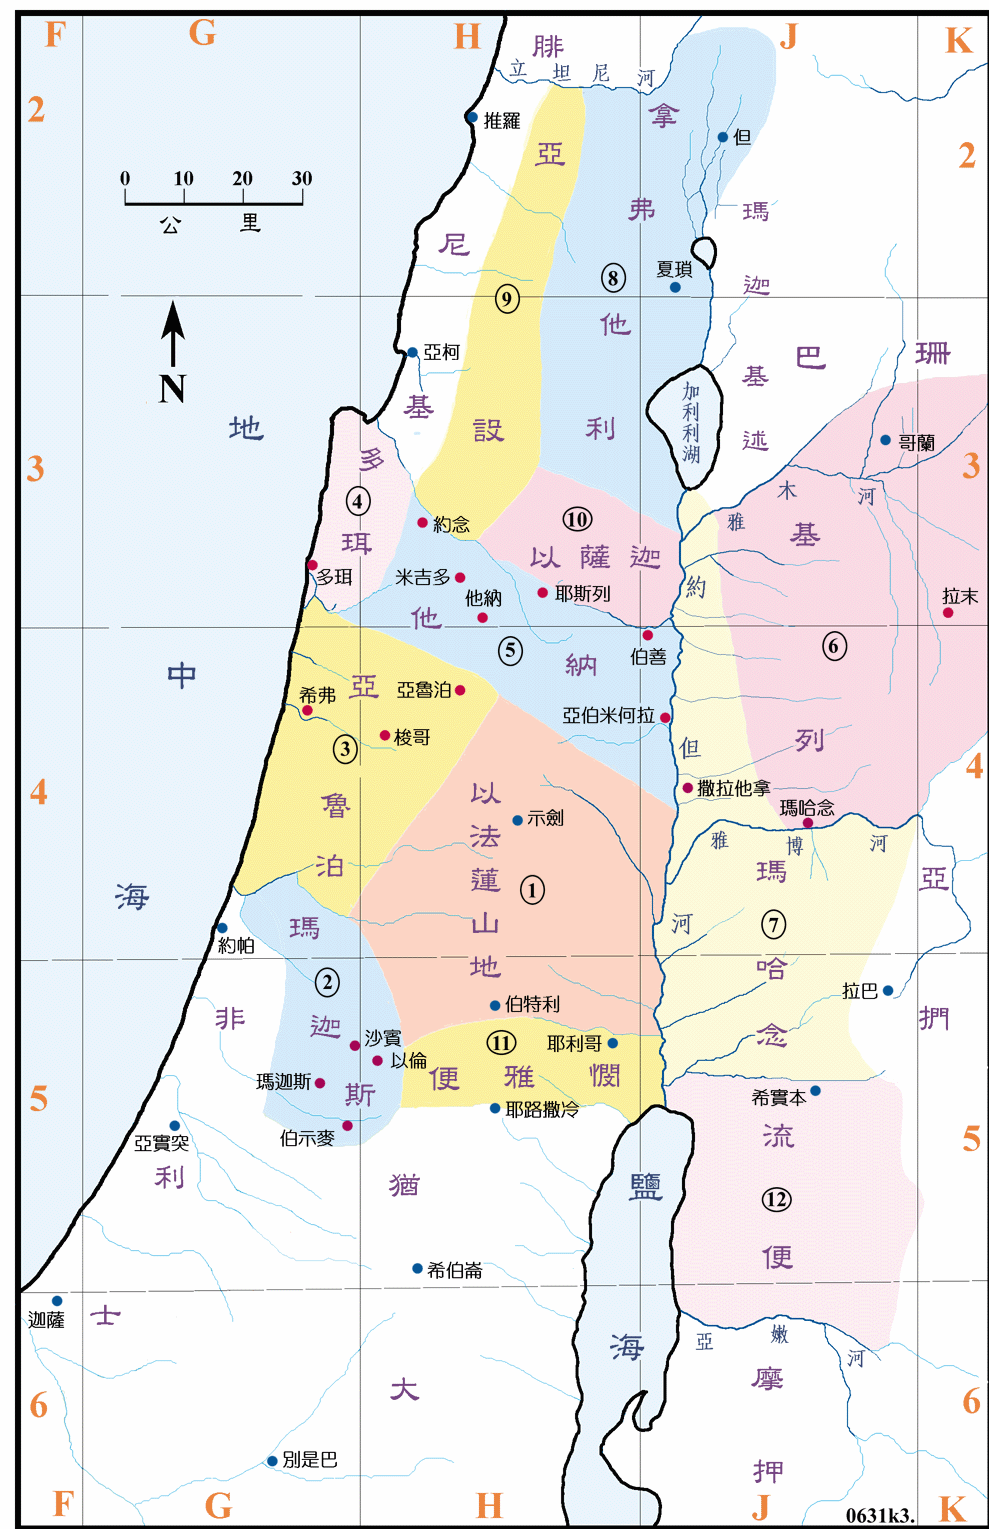
\includegraphics[width=6in]{BLiShiFigs/king/bantu}
\caption{所羅門時期的版圖}
\label{fig:sub1}
\end{figure}%
 24 所羅門管理大河西邊的諸王，以及從提弗薩直到加沙的全地，四境盡都平安。 25 所羅門在世的日子，從但到別是巴的猶大人和以色列人，都在自己的葡萄樹下和無花果樹下安然居住。 26 所羅門有套車的馬四萬，還有馬兵一萬二千。 27 那十二個官吏各按各月供給所羅門王，並一切與他同席之人的食物，一無所缺。 28 眾人各按各分，將養馬與快馬的大麥和乾草送到官吏那裡。

\subsubsection{所羅門之智能  4:29-34}
神賜給所羅門極大的智慧、聰明和廣大的心，如同海沙不可測量。 30 所羅門的智慧超過東方人和埃及人的一切智慧。 31 他的智慧勝過萬人，勝過以斯拉人以探並瑪曷的兒子希幔、甲各、達大的智慧。他的名聲傳揚在四圍的列國。 32 他作箴言三千句，詩歌一千零五首。 33 他講論草木，自黎巴嫩的香柏樹直到牆上長的牛膝草，又講論飛禽走獸、昆蟲水族。 34 天下列王聽見所羅門的智慧，就都差人來聽他的智慧話。


\subsection{所羅門建殿 5-8 }
\subsubsection{與希蘭王立約建殿 5:1-11}
\begin{table}[!hbp]
\centering
\begin{tabular}{p{9cm}|p{8cm}}\hline\hline
所羅門&推羅王希蘭\\\hline\hline
&推羅王希蘭平素愛大衛，他聽見以色列人膏所羅門，接續他父親做王，就差遣臣僕來見他。\\\hline
所羅門也差遣人去見希蘭，說： 3 「你知道我父親大衛因四圍的爭戰，不能為耶和華他神的名建殿，直等到耶和華使仇敵都服在他腳下。 4 現在耶和華我的神使我四圍平安，沒有仇敵，沒有災禍。 5 我定意要為耶和華我神的名建殿，是照耶和華應許我父親大衛的話說：『我必使你兒子接續你坐你的位，他必為我的名建殿。』 6 所以求你吩咐你的僕人在黎巴嫩為我\textcolor{blue}{砍伐香柏木}，我的僕人也必幫助他們，我必照你所定的，給你僕人的工價。因為你知道，在我們中間沒有人像西頓人善於砍伐樹木。」&希蘭聽見所羅門的話，就甚喜悅，說：「今日應當稱頌耶和華！因他賜給大衛一個有智慧的兒子，治理這眾多的民。」 8 希蘭打發人去見所羅門，說：「你差遣人向我所提的那事，我都聽見了。論到香柏木和松木，我必照你的心願而行。 9 我的僕人必將這木料從黎巴嫩運到海裡，紮成筏子，浮海運到你所指定我的地方，在那裡拆開，你就可以收取。你也要成全我的心願，將\textcolor{blue}{食物給我的家}。」於是希蘭照著所羅門所要的，給他香柏木和松木。\\\hline
所羅門給希蘭麥子二萬歌珥，清油二十歌珥，做他家的食物，所羅門每年都是這樣給希蘭。&\\\hline
\end{tabular}
\caption{所羅門建殿的準備}
\end{table}


\subsubsection{所羅門建殿的準備工 5:12-18}
\begin{wraptable}{r}{10cm}\vspace*{-10mm}
\centering
\begin{tabular}{p{1.5cm}|p{2cm}|p{5.4cm}}\hline\hline
預備的人&數量 &地點　\\\hline\hline
扛抬工人    &70,000    &以色列地所有寄居的外邦人 \\\hline
鑿石工人  &80,000名 &以色列地所有寄居的外邦人 \\\hline
督工          &3,300    &以色列地所有寄居的外邦人  \\\hline
服苦的人 &30,000輪流 &1000/月上利巴嫩；兩個月在家裡\\\hline
\end{tabular}
\caption{所羅門建殿的準備}
\end{wraptable}
12 耶和華照著所應許的賜智慧給所羅門。希蘭與所羅門和好，彼此立約。13 所羅門王從以色列人中挑取服苦的人共有三萬， 14 派他們輪流每月一萬人上黎巴嫩去，一個月在黎巴嫩，兩個月在家裡，亞多尼蘭掌管他們。 15 所羅門用七萬扛抬的，八萬在山上鑿石頭的。 16 此外，所羅門用三千三百督工的，監管工人。 17 王下令，人就鑿出又大又寶貴的石頭來，用以立殿的根基。 18 所羅門的匠人和希蘭的匠人並迦巴勒人，都將石頭鑿好，預備木料和石頭建殿。

\subsubsection{所羅門建殿的細節 6-7 }
\begin{table}[H]\centering
\begin{tabular}{p{2cm}|p{15.cm}}\hline\hline
位置      &方法    \\\hline\hline
 殿   & 長寬高=60x20x30肘,殿安置香柏木的棟梁，又用香柏木板遮蓋.殿裡面用香柏木板貼牆，從地到棚頂都用木板遮蔽，又用松木板鋪地.香柏木上面刻著野瓜和初開的花,全殿都貼上金子\\\hline
 內殿& 長寬高=20x20x30肘.就是至聖所，從地到棚頂用香柏木板遮蔽,牆面都貼上精金,內、外殿的地板都貼上金子\\\hline
 外殿& 長寬高=40x20x30肘,精金貼了殿內的牆\\\hline
殿前的廊子   & 長寬闊=20x20x10肘  \\\hline
窗櫺    & 為殿做了嚴緊的窗櫺\\\hline
旁屋& 靠著殿牆，圍著外殿內殿，造了三層旁屋,下層寬五肘，中層寬六肘，上層寬七肘,殿右邊當中的旁屋有門，門內有旋螺的樓梯，可以上到第二層，從第二層可以上到第三層.每層高五肘，香柏木的棟梁擱在殿牆坎上\\\hline
壇& 用香柏木做壇，包上精金 \\\hline
內殿門扇、門楣、門框& 用橄欖木製造,門口有牆的五分之一,都貼上金子 \\\hline
門框& 用橄欖木製造外殿的門框，門口有牆的四分之一\\\hline
門& 用松木做門兩扇。這扇分兩扇，是摺疊的；那扇分兩扇；也是摺疊的\\\hline
內院& 用鑿成的石頭三層、香柏木一層建築\\\hline
 內殿    & 用橄欖木做兩個基路伯，各高十肘.路伯有兩個翅膀，各長五肘，從這翅膀尖到那翅膀尖共有十肘,高十肘.基路伯的翅膀是張開的，這基路伯的一個翅膀挨著這邊的牆，那基路伯的一個翅膀挨著那邊的牆，裡邊的兩個翅膀在殿中間彼此相接.用金子包裹二基路伯    \\\hline
內外殿的牆上   & 刻著基路伯、棕樹，和初開的花   \\\hline
兩門扇上   & 在橄欖木做的兩門扇上刻著基路伯、棕樹，和初開的花，都貼上金子\\\hline
盆座撐子和心子上 & 刻著基路伯、獅子，和棕樹，周圍有瓔珞\\\hline
\end{tabular}
\caption{神的殿}
\end{table}

\subsubsection{始建聖殿 6:1-10}
\begin{figure}[ht]
\begin{subfigure}{.5\textwidth}
  \centering
  % include first image
  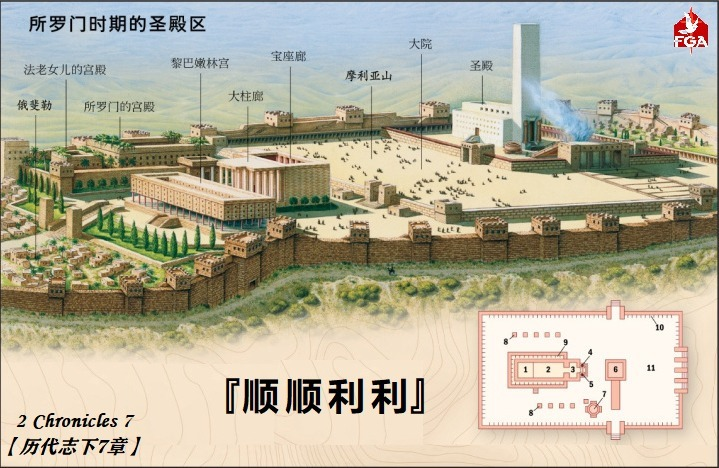
\includegraphics[width=.9\textwidth]{BLiShiFigs/king/temple}  
  \caption{聖殿全貌}
 % \label{fig:sub-first}
\end{subfigure}
\begin{subfigure}{.5\textwidth}
  \centering
  % include second image
  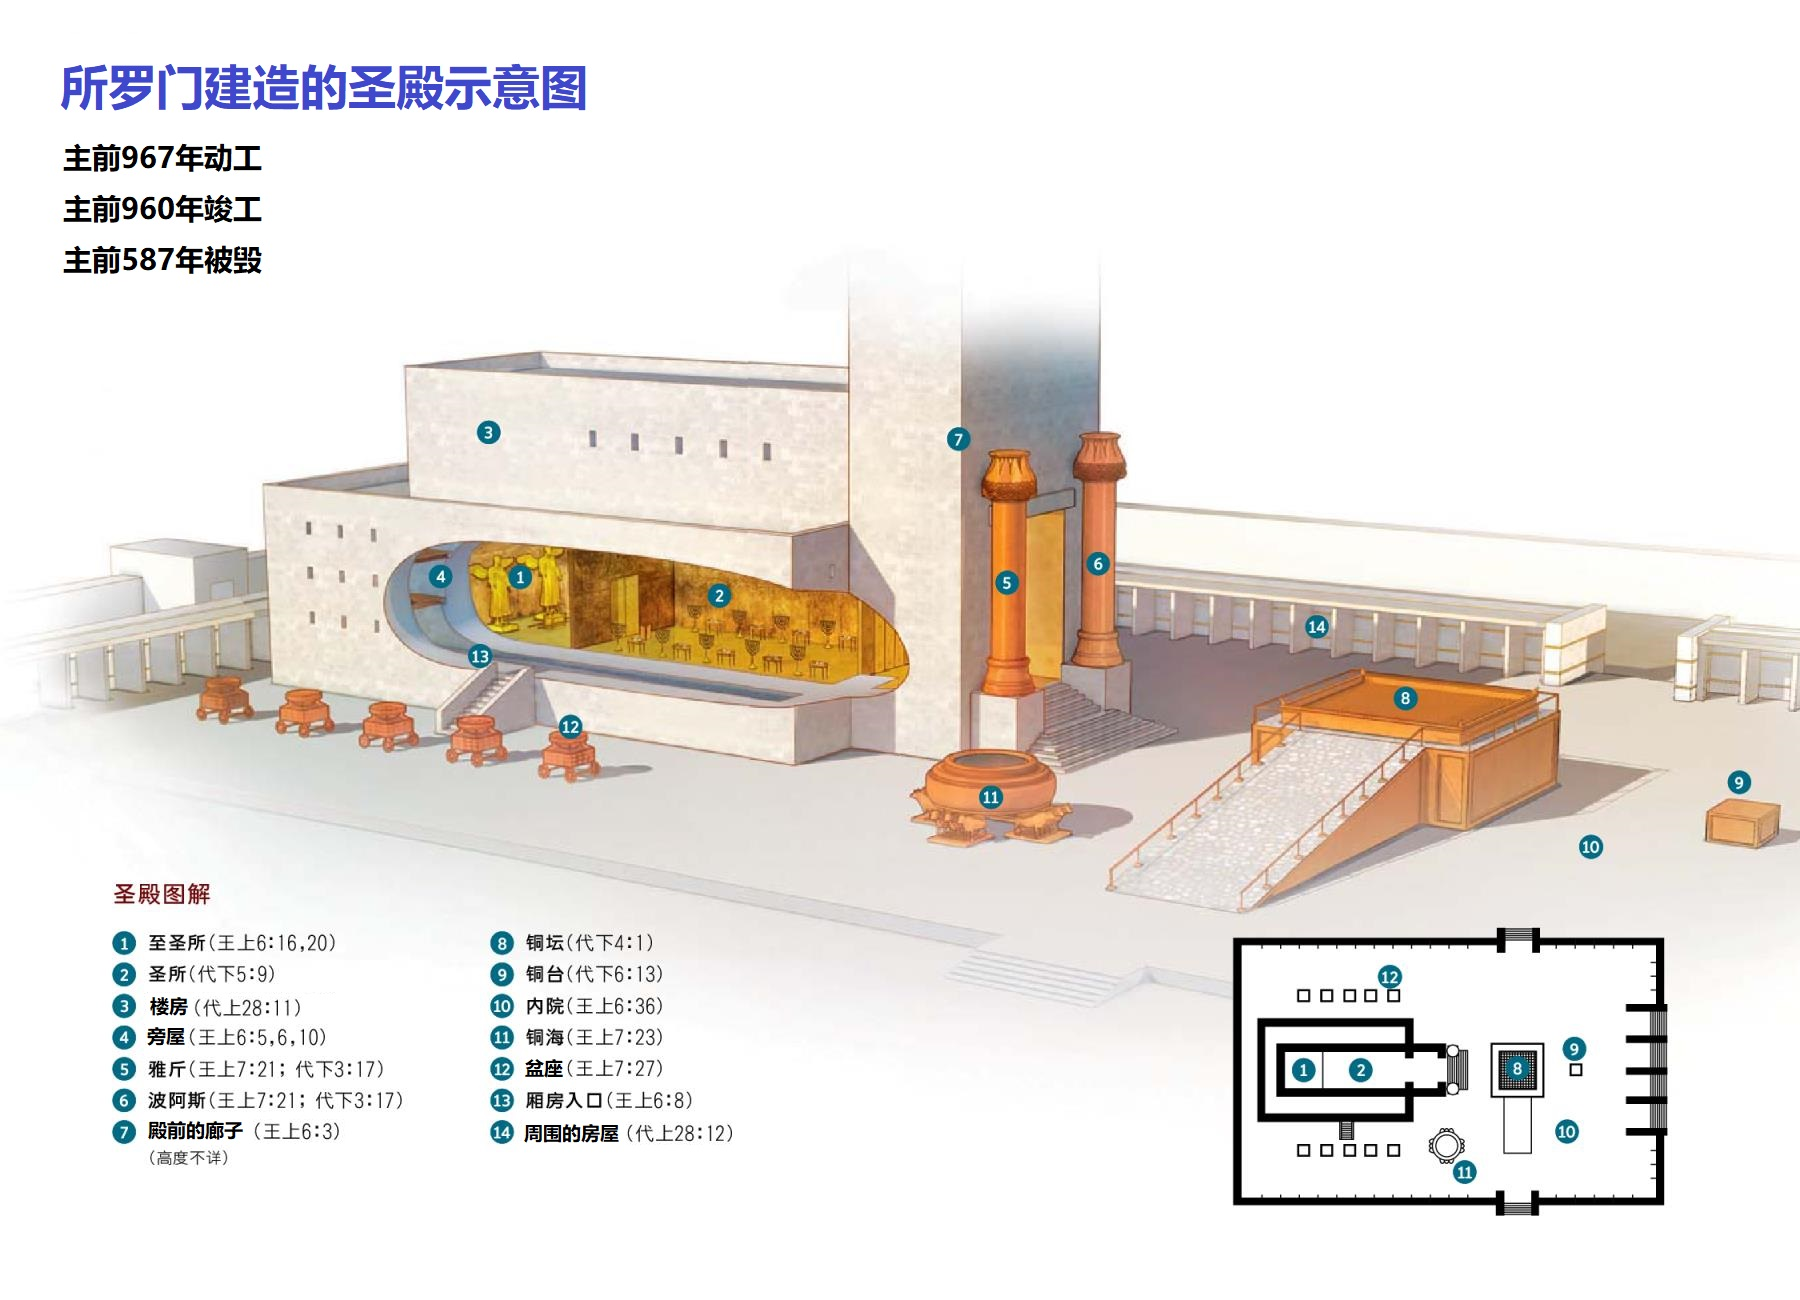
\includegraphics[width=.9\textwidth]{BLiShiFigs/king/solomonetemple}  
  \caption{聖殿示意图}
  \label{fig:sub-second}
\end{subfigure}
\label{fig:fig}
\end{figure}


\begin{table}[!hbp]
\centering 
\begin{tabular}{|p{1cm}|p{3.5cm}|p{7.5cm}|p{3cm}|}\hline\hline
 &猶太曆 &		節期 &	西曆 \\\hline\hline
1&尼散月或亞筆月&逾越節&	三至四月間\\\hline
2&以珥月&補逾越節&	四至五月間\\\hline
3&西彎月& 七七節（五旬節）&	五至六月間\\\hline
4&搭模斯月&		&六至七月間\\\hline
5&埃波月	&	&七至八月間\\\hline
6&以祿月&&		八至九月間\\\hline
7&提斯利月或以他念月	& 吹角節、10 贖罪日、15-21 住棚節、22 嚴肅會	&九至十月間\\\hline
8&瑪西班月&	&十至十一月間\\\hline
9&基斯流月& 提別月修殿節	&十一至十二月間\\\hline
10  &提別月  &	&十二至一月間\\\hline
11  &細罷特月&	&一月至二月間\\\hline
12L &第一亞達月2&&	二至三月間\\\hline
12 &亞達月／第二亞達月& 普珥節&\\\hline
\end{tabular}
\caption{猶太曆及西曆}
\end{table}
\begin{figure}[ht]
\begin{subfigure}{.5\textwidth}
  \centering
  % include first image
  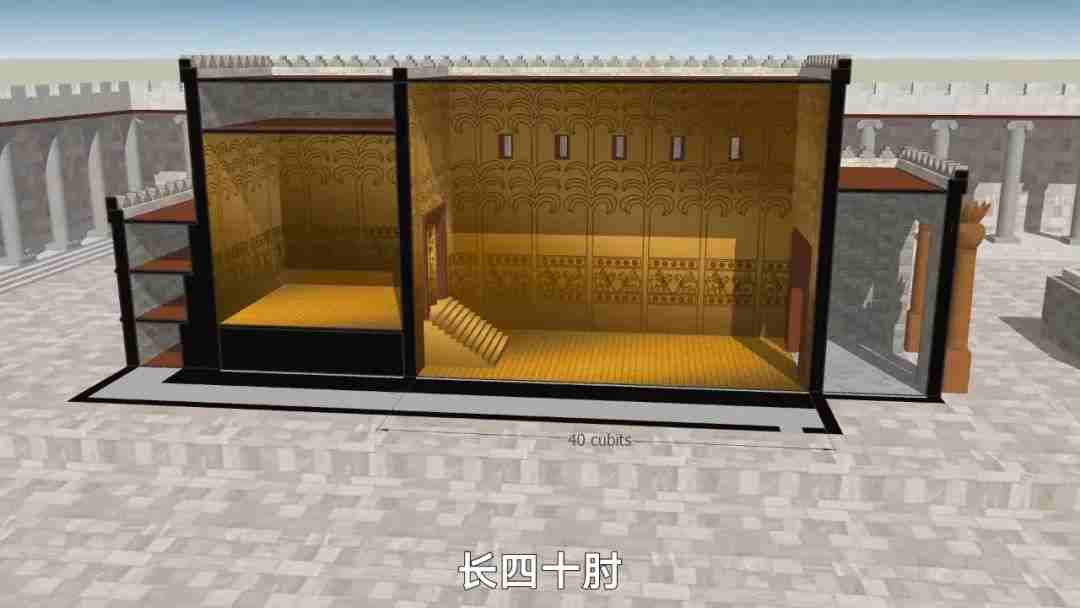
\includegraphics[width=.9\textwidth]{BLiShiFigs/king/internal}  
  \caption{内部结构}
 % \label{fig:sub-first}
\end{subfigure}
\begin{subfigure}{.5\textwidth}
  \centering
  % include second image
  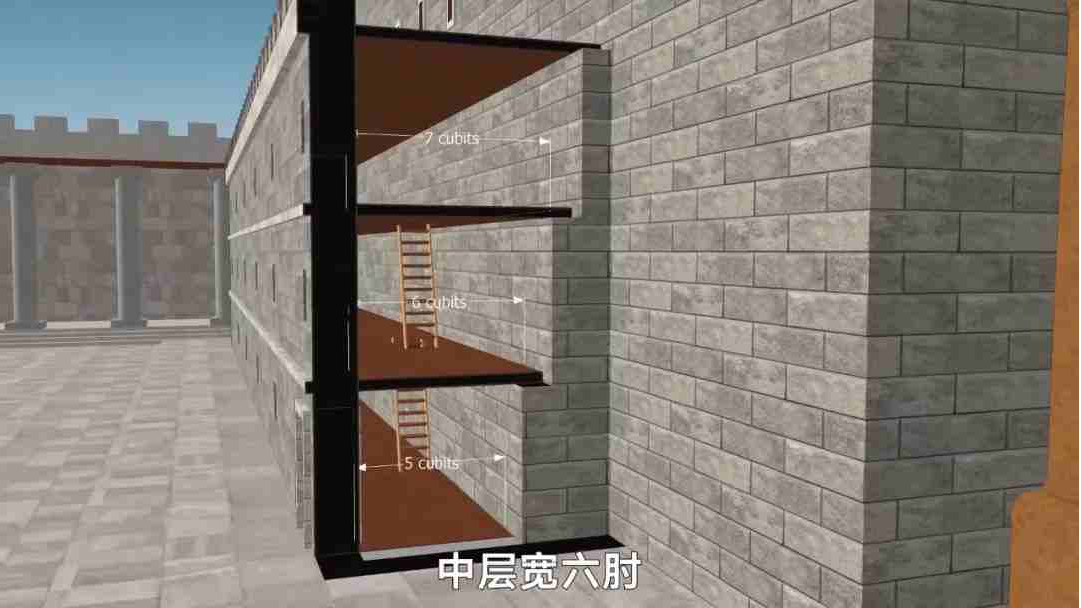
\includegraphics[width=.9\textwidth]{BLiShiFigs/king/level}  
  \caption{三层示意图}
  \label{fig:sub-second}
\end{subfigure}
\label{fig:fig}
\end{figure}
以色列人出埃及地後四百八十年，所羅門做以色列王第四年西弗月，就是二月，開工建造耶和華的殿。 2 所羅門王為耶和華所建的殿，長六十肘，寬二十肘，高三十肘。 3 殿前的廊子長二十肘，與殿的寬窄一樣，闊十肘。 4 又為殿做了嚴緊的窗櫺。 5 靠著殿牆，圍著外殿、內殿，造了三層旁屋， 6 下層寬五肘，中層寬六肘，上層寬七肘。殿外旁屋的梁木擱在殿牆坎上，免得插入殿牆。 7 建殿是用山中鑿成的石頭，建殿的時候，\textcolor{blue}{錘子、斧子和別樣鐵器的響聲都沒有聽見}。 8 在殿右邊當中的旁屋有門，門內有旋螺的樓梯，可以上到第二層，從第二層可以上到第三層。 9 所羅門建殿，安置香柏木的棟梁，又用香柏木板遮蓋。 10 靠著殿所造的旁屋，每層高五肘，香柏木的棟梁擱在殿牆坎上。

\subsubsection{耶和華向所羅門之約 6:11-13}
\begin{table}[H]
\centering
\begin{tabular}{p{8.5cm}|p{7.5cm}}\hline\hline
所羅門若遵行&耶和華必應驗\\\hline\hline
耶和華的話臨到所羅門說：「論到你所建的這殿，\textcolor{blue}{你若遵行}我的律例，謹守我的典章，遵從我的一切誡命， &\textcolor{blue}{我必向你應驗}我所應許你父親大衛的話。我必住在以色列人中間，並不丟棄我民以色列。」\\\hline
\end{tabular}
\caption{耶和華之約}
\end{table}


\subsubsection{造內殿 6:14-22}
\begin{wrapfigure}{r}{0.4\textwidth}
\centering
\vspace{-10mm}
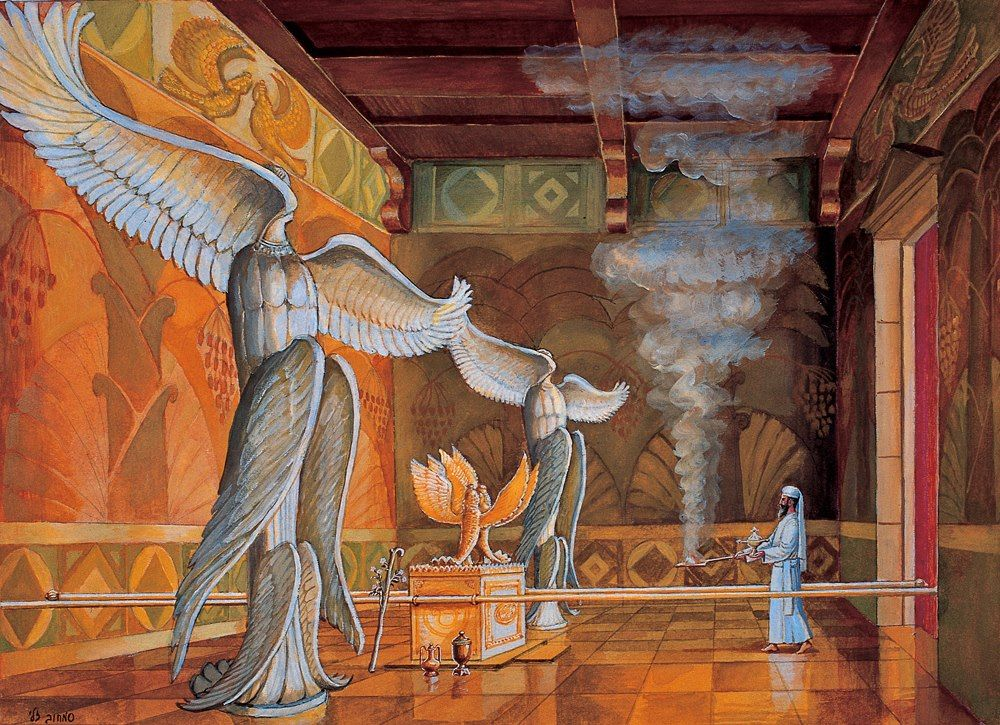
\includegraphics[width=2.8in]{BLiShiFigs/king/holytemple}
\caption{造內殿}
\label{fig:sub1}
\end{wrapfigure}
所羅門建造殿宇。 15 殿裡面用香柏木板貼牆，從地到篷頂都用木板遮蔽，又用松木板鋪地。 16 內殿，就是至聖所，長二十肘，從地到篷頂用香柏木板遮蔽(隔斷)。 17 內殿前的外殿，長四十肘。 18 殿裡一點石頭都不顯露，一概用香柏木遮蔽，上面刻著野瓜和初開的花。 19 殿裡預備了內殿，好安放耶和華的約櫃。 20 內殿長二十肘，寬二十肘，高二十肘，牆面都貼上精金。又用香柏木做壇，包上精金。 21 所羅門用精金貼了殿內的牆，又用金鏈子掛在內殿前門扇，用金包裹。 22 全殿都貼上金子，直到貼完。內殿前的壇，也都用金包裹。


\subsubsection{建造內殿的基路伯 6:23-28} 
\begin{wrapfigure}{r}{0.4\textwidth}
\centering
\vspace{-10mm}
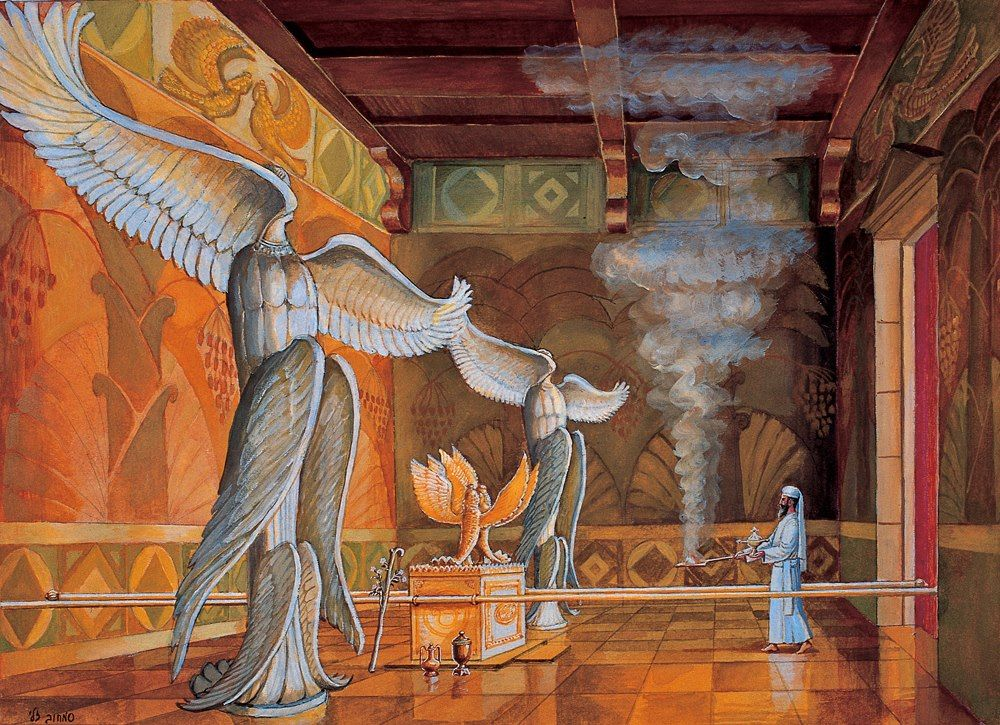
\includegraphics[width=2.8in]{BLiShiFigs/king/holytemple}
\caption{內殿的基路伯}
\label{fig:sub1}
\end{wrapfigure}
他用橄欖木做兩個基路伯，各高十肘，安在內殿。 24 這一個基路伯有兩個翅膀，各長五肘，從這翅膀尖到那翅膀尖共有十肘。 25 那一個基路伯的兩個翅膀也是十肘，兩個基路伯的尺寸、形象都是一樣。 26 這基路伯高十肘，那基路伯也是如此。 27 他將兩個基路伯安在內殿裡，基路伯的翅膀是張開的，這基路伯的一個翅膀挨著這邊的牆，那基路伯的一個翅膀挨著那邊的牆，裡邊的兩個翅膀在殿中間彼此相接。 28 又用金子包裹二基路伯。

\subsubsection{殿之裝飾 6:29-38}
內殿、外殿周圍的牆上都刻著基路伯、棕樹和初開的花。 30 內殿、外殿的地板都貼上金子。 31 又用橄欖木製造內殿的門扇、門楣、門框，門口有牆的五分之一。 32 在橄欖木做的兩門扇上刻著基路伯、棕樹和初開的花，都貼上金子。 33 又用橄欖木製造外殿的門框，門口有牆的四分之一。 34 用松木做門兩扇，這扇分兩扇，是摺疊的，那扇分兩扇，也是摺疊的。 35 上面刻著基路伯、棕樹和初開的花，都用金子貼了。 36 他又用鑿成的石頭三層，香柏木一層建築內院。

37 所羅門在位第四年西弗月，立了耶和華殿的根基。 38 到十一年布勒月，就是八月，殿和一切屬殿的都按著樣式造成。他建殿的工夫共有七年。


\subsubsection{建黎巴嫩林宮 7:1-12}
所羅門為自己建造宮室，十三年方才造成。 2 又建造黎巴嫩林宮，長一百肘，寬五十肘，高三十肘。有香柏木柱三(四)行，柱上有香柏木柁梁， 3 其上以香柏木為蓋，每行柱子十五根，共有四十五根。 4 有窗戶三層，窗與窗相對。 5 所有的門框都是厚木見方的，有窗戶三層，窗與窗相對。 6 並建造有柱子的廊子，長五十肘，寬三十肘。在這廊前又有廊子，廊外有柱子和臺階。 7 又建造一廊，其中設立審判的座位，這廊從地到頂都用香柏木遮蔽。 8 廊後院內有所羅門住的宮室，工作與這工作相同。所羅門又為所娶法老的女兒建造一宮，做法與這廊子一樣。

9 建造這一切所用的石頭都是寶貴的，是按著尺寸鑿成的，是用鋸裡外鋸齊的。從根基直到簷石，從外頭直到大院，都是如此。 10 根基是寶貴的大石頭，有長十肘的，有長八肘的， 11 上面有香柏木和按著尺寸鑿成寶貴的石頭。 12 大院周圍有鑿成的石頭三層，香柏木一層，都照耶和華殿的內院和殿廊的樣式。

\subsubsection{拿弗他利寡婦,推羅人戶蘭之銅技 7:13-14}
\begin{wraptable}{r}{10cm}
\centering
\begin{tabular}{p{2.5cm}|p{7cm}}\hline\hline
名稱      & 備註   \\\hline\hline
銅柱子  &兩根，每根高十八肘，圍十二肘\\\hline
柱頂&用銅鑄了兩個柱頂安在柱上，各高五肘\\\hline
銅海   &圓的，高五xx徑十xx圍三十肘,在海邊之下 \\\hline
銅牛  & 有十二隻銅牛馱海，可容二千罷特 \\\hline
盆座&每座長寬高4x4x3肘,四面都有心子\\\hline
盆&每盆可容四十罷特。盆徑四肘 \\\hline
盆、鏟子，盤子&用光亮的銅\\\hline
\end{tabular}
\caption{戶蘭造銅器具}
\end{wraptable}
所羅門王差遣人往推羅去，將戶蘭召了來。 14 他是拿弗他利支派中一個寡婦的兒子，他父親是推羅人，做銅匠的。戶蘭滿有智慧、聰明、技能，善於各樣銅作。他來到所羅門王那裡，做王一切所要做的。

\subsubsection{製銅柱 7:15-22}
他製造兩根銅柱，每根高十八肘，圍十二肘。 16 又用銅鑄了兩個柱頂安在柱上，各高五肘。 17 柱頂上有裝修的網子和擰成的鏈索，每頂七個。 18 網子周圍有兩行石榴遮蓋柱頂，兩個柱頂都是如此。 19 廊子的柱頂徑四肘，刻著百合花。 20 兩柱頂的鼓肚上挨著網子，各有兩行石榴環繞，兩行共有二百。 21 他將兩根柱子立在殿廊前頭，右邊立一根，起名叫雅斤，左邊立一根，起名叫波阿斯。 22 在柱頂上刻著百合花。這樣，造柱子的工就完畢了。


\subsubsection{鑄銅海 7:23-26}
\begin{wrapfigure}{r}{0.4\textwidth}
\centering
\vspace{-10mm}
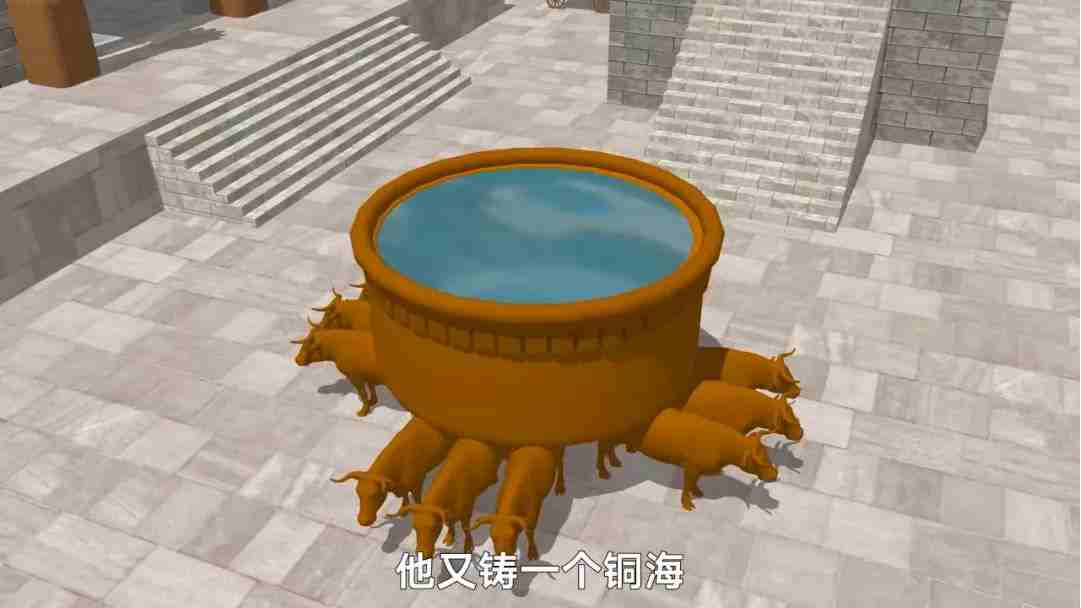
\includegraphics[width=2.8in]{BLiShiFigs/king/copper}
\caption{鑄銅海}
\label{fig:sub1}
\end{wrapfigure}
他又鑄一個銅海，樣式是圓的，高五肘，徑十肘，圍三十肘。 24 在海邊之下，周圍有野瓜的樣式，每肘十瓜，共有兩行，是鑄海的時候鑄上的。 25 有十二隻銅牛馱海，三隻向北，三隻向西，三隻向南，三隻向東。海在牛上，牛尾都向內。 26 海厚一掌，邊如杯邊，又如百合花，可容二千罷特。

\subsubsection{製銅座 7:27-36}
他用銅製造十個盆座，每座長四肘，寬四肘，高三肘。 28 座的造法是這樣：四面都有心子，心子在邊子當中。 29 心子上有獅子和牛並基路伯。邊上有小座，獅子和牛以下有垂下的瓔珞。 30 每盆座有四個銅輪和銅軸。小座的四角上在盆以下，有鑄成的盆架，其旁都有瓔珞。 31 小座高一肘，口是圓的，彷彿座的樣式，徑一肘半，在口上有雕工，心子是方的，不是圓的。 32 四個輪子在心子以下，輪軸與座相連，每輪高一肘半。 33 輪的樣式如同車輪，軸、輞、輻、轂都是鑄的。 34 每座四角上都有盆架，是與座一同鑄成的。 35 座上有圓架，高半肘。座上有撐子和心子，是與座一同鑄的。 36 在撐子和心子上刻著基路伯、獅子和棕樹，周圍有瓔珞。 37 十個盆座都是這樣，鑄法、尺寸、樣式相同。

\subsubsection{製銅盆 7:38-47}
又用銅製造十個盆，每盆可容四十罷特，盆徑四肘。在那十座上，每座安設一盆。 39 五個安在殿門的右邊，五個放在殿門的左邊。又將海放在殿門的右旁，就是南邊。 40 戶蘭又造了盆、鏟子和盤子。這樣，他為所羅門王做完了耶和華殿的一切工。 41 所造的就是兩根柱子和柱上兩個如球的頂，並兩個蓋柱頂的網子， 42 和四百石榴，安在兩個網子上，每網兩行，蓋著兩個柱上如球的頂。 43 十個座和其上的十個盆， 44 海和海下的十二隻牛， 45 盆、鏟子、盤子。這一切都是戶蘭給所羅門王用光亮的銅為耶和華的殿造成的， 46 是遵王命在約旦平原，疏割和撒拉但中間藉膠泥鑄成的。 47 這一切所羅門都沒有過秤，因為甚多，銅的輕重也無法可查。

\subsubsection{造其他的殿裡器皿,殿工告竣 7:48-51}
\begin{wraptable}{r}{7cm}
\vspace{-5mm}
\centering 
\begin{tabular}{p{4.5cm}|p{2cm}}
\hline
\hline
金壇    & 神殿裡的\\\hline
金桌子  &  陳設餅\\\hline
金燈臺& 內殿前\\\hline
燈上的金花、燈盞、蠟剪&外殿\\\hline
金杯,盤,鑷子,調羹,火鼎&外殿\\\hline
門樞&內殿,外殿\\\hline
\end{tabular}
\caption{殿中的金器具}
\end{wraptable}
所羅門又造耶和華殿裡的金壇和陳設餅的金桌子； 49 內殿前的精金燈臺，右邊五個，左邊五個；並其上的金花、燈盞、蠟剪； 50 與精金的杯、盤、鑷子、調羹、火鼎；以及至聖所，內殿的門樞和外殿的門樞。所羅門王做完了耶和華殿的一切工，就把他父大衛分別為聖的金銀和器皿都帶來，放在耶和華殿的府庫裡。


\subsubsection{以他念月在節前運送聖器具及約櫃 8:1-11}
\begin{table}[H]
\centering 
\begin{tabular}{p{4.cm}|p{11.25cm}|p{2.2cm}}\hline\hline
眾人聚集到所羅門王那裡&抬約櫃進內殿&耶和華的榮光\\\hline
\multirow{4}{4.1cm}{那時，所羅門將以色列的長老和各支派的首領並以色列的族長，招聚到耶路撒冷，要把耶和華的約櫃從大衛城就是錫安運上來。以他念月，就是七月，在節前，以色列人都聚集到所羅門王那裡。}
&以色列長老來到，祭司便抬起約櫃，祭司和利未人將耶和華的約櫃運上來，又將會幕和會幕的一切聖器具都帶上來。
&\multirow{4}{2.3cm}{祭司從聖所出來的時候，有雲充滿耶和華的殿，甚至祭司不能站立供職，因為耶和華的榮光充滿了殿。}\\\cline{2-2}
&所羅門王和聚集到他那裡的以色列全會眾，一同在約櫃前獻牛羊為祭，多得不可勝數。&\\\cline{2-2}
&祭司將耶和華的約櫃抬進內殿，就是至聖所，放在兩個基路伯的翅膀底下。基路伯張著翅膀在約櫃之上，遮掩約櫃和抬櫃的槓。這槓甚長，槓頭在內殿前的聖所可以看見，在殿外卻不能看見，直到如今還在那裡。&\\\cline{2-2}
&約櫃裡唯有兩塊石版，就是以色列人出埃及地後，耶和華與他們立約的時候，摩西在何烈山所放的，除此以外，並無別物。&\\\hline
\end{tabular}
\caption{運送聖器具及約櫃}
\end{table}

\subsubsection{所羅門宣述建殿之來由 8:14-21}
\begin{table}[H]
\centering 
\begin{tabular}{p{3.3cm}|p{5.1cm}|p{8.75cm}}\hline\hline
%&&\\\hline
那時所羅門說：「耶和華曾說他必住在幽暗之處。我已經建造殿宇做你的居所，為你永遠的住處。」王轉臉為以色列會眾祝福，以色列會眾就都站立。
&所羅門說：「耶和華以色列的神是應當稱頌的！因他親口向我父大衛所應許的，也親手成就了。他說：『自從我領我民以色列出埃及以來，我未曾在以色列各支派中選擇一城建造殿宇為我名的居所，但揀選大衛治理我民以色列。』」&所羅門說：「我父大衛曾立意要為耶和華以色列神的名建殿，耶和華卻對我父大衛說：『你立意為我的名建殿，這意思甚好，只是你不可建殿，唯你所生的兒子必為我名建殿。』現在耶和華成就了他所應許的話，使我接續我父大衛坐以色列的國位，又為耶和華以色列神的名建造了殿。我也在其中為約櫃預備一處，約櫃內有耶和華的約，就是他領我們列祖出埃及地的時候，與他們所立的約。」\\\hline
\end{tabular}
\caption{運送聖器具及約櫃}
\end{table}

\subsubsection{求耶和華應允禱告 8:22-30}
\begin{table}[H]
\vspace{-5mm}
\centering 
\begin{tabular}{p{5.3cm}|p{5.1cm}|p{7.2cm}}\hline\hline
現在應驗的應許&求神應驗的&求神垂聽民向此處的祈禱\\\hline
所羅門當著以色列會眾，站在耶和華的壇前，向天舉手說：「耶和華以色列的神啊，天上地下，沒有神可比你的。你向那盡心行在你面前的僕人守約施慈愛，向你僕人我父大衛所應許的話現在應驗了。你親口應許，親手成就，正如今日一樣。
&耶和華以色列的神啊，你所應許你僕人我父大衛的話說『你的子孫若謹慎自己的行為，在我面前行事像你所行的一樣，就不斷人坐以色列的國位』，現在求你應驗這話。以色列的神啊，求你成就向你僕人我父大衛所應許的話！
&神果真住在地上嗎?看哪，天和天上的天尚且不足你居住的，何況我所建的這殿呢!唯求耶和華我的神垂顧僕人的禱告,祈求，俯聽僕人今日在你面前的祈禱,呼籲。願你晝夜看顧這殿，就是你應許立為你名的居所；求你垂聽僕人向此處禱告的話。你僕人和你民以色列向此處祈禱的時候求你在天上你的居所垂聽，垂聽而赦免\\\hline
\end{tabular}
\caption{求耶和華應允禱告}
\end{table}



\subsubsection{所羅門禱告的各種境況 8:31-53}
\begin{table}[!hbp]
\vspace{-7mm}
\centering 
\begin{tabular}{p{3.75cm}|p{4.65cm}|p{8.5cm}}\hline\hline
各種境況 & 禱告蒙應允的條件 & 向神的祈求\\\hline\hline
人若得罪鄰舍，有人叫他起誓&他來到這殿，在你的壇前起誓&求你從天上垂聽，判斷你的僕人，定惡人有罪，照他所行的報應在他頭上；定義人有理，照他的義賞賜他。\\\hline
你的民以色列若得罪你，敗在仇敵面前&又歸向你，承認你的名，在這殿裡祈求、禱告，&求你從天上垂聽，赦免你民以色列的罪，使他們歸回你賜給他們和他們列祖之地\\\hline
你的民因得罪你，你懲罰他們，使天閉塞不下雨&他們若向此處禱告，承認你的名，離開他們的罪&求你在天上垂聽，赦免你僕人和你民以色列的罪，將當行的善道指教他們，且降雨在你的地，就是你賜給你民為業之地\\\hline
國中若有饑荒、瘟疫、旱風、霉爛、蝗蟲、螞蚱，或有仇敵犯境，圍困城邑，無論遭遇什麼災禍疾病&你的民以色列，或是眾人，或是一人，自覺有罪 (災禍)，向這殿舉手，無論祈求什麼，禱告什麼&求你從天上你的居所垂聽赦免。你是知道人心的，要照各人所行的待他們—唯有你知道世人的心—使他們在你賜給我們列祖之地上一生一世敬畏你。\\\hline
論到不屬你民以色列的外邦人&為你名從遠方而來—他們聽人論說你的大名和大能的手並伸出來的膀臂—向這殿禱告&求你在天上你的居所垂聽，照著外邦人所祈求的而行，使天下萬民都認識你的名，敬畏你，像你的民以色列一樣，又使他們知道我建造的這殿是稱為你名下的。\\\hline
你的民若奉你的差遣，無論往何處去與仇敵爭戰&向耶和華所選擇的城與我為你名所建造的殿禱告&求你在天上垂聽他們的禱告、祈求，使他們得勝\\\hline
你的民若得罪你（世上沒有不犯罪的人），你向他們發怒，將他們交給仇敵擄到仇敵之地，或遠或近&他們若在擄到之地想起罪來，回心轉意，懇求你說『我們有罪了，我們悖逆了，我們作惡了』，他們若在擄到之地盡心、盡性歸服你，又向自己的地，就是你賜給他們列祖之地，和你所選擇的城，並我為你名所建造的殿禱告，&求你在天上你的居所垂聽他們的禱告、祈求，為他們申冤，饒恕得罪你的民，赦免他們的一切過犯，使他們在擄他們的人面前蒙憐恤，因為他們是你的子民，你的產業，是你從埃及領出來脫離鐵爐的。願你的眼目看顧僕人，聽你民以色列的祈求，無論何時向你祈求，願你垂聽。主耶和華啊，你將他們從地上的萬民中分別出來做你的產業，是照你領我們列祖出埃及的時候，藉你僕人摩西所應許的話。\\\hline
\end{tabular}
\caption{所羅門禱告的各種境況}
\end{table}

\subsubsection{為民祝福 8:54-61}
所羅門在耶和華的壇前屈膝跪著，向天舉手，在耶和華面前禱告祈求已畢，就起來， 55 站著，大聲為以色列全會眾祝福，說： 56 「耶和華是應當稱頌的！因為他照著一切所應許的賜平安給他的民以色列人，凡藉他僕人摩西應許賜福的話，一句都沒有落空。 57 願耶和華我們的神與我們同在，像與我們列祖同在一樣，不撇下我們，不丟棄我們， 58 使我們的心歸向他，遵行他的道，謹守他吩咐我們列祖的誡命、律例、典章。 59 我在耶和華面前祈求的這些話，願耶和華我們的神晝夜垂念，每日為他僕人與他民以色列申冤， 60 使地上的萬民都知道唯獨耶和華是神，並無別神。 61 所以你們當向耶和華我們的神存誠實的心，遵行他的律例，謹守他的誡命，至終如今日一樣。」

\subsubsection{獻殿禮 8:62-66}
\begin{table}[H]
\vspace{-3mm}
\centering 
\begin{tabular}{p{9.2cm}|p{8.45cm}}\hline\hline
獻祭&眾人聚集十四日,心中喜樂\\\hline\hline
王和以色列眾民一同在耶和華面前獻祭。所羅門向耶和華獻平安祭，用牛二萬二千，羊十二萬。這樣王和以色列眾民為耶和華的殿行奉獻之禮。當日王因耶和華殿前的銅壇太小，容不下燔祭、素祭和平安祭牲的脂油，便將耶和華殿前院子當中分別為聖，在那裡獻燔祭、素祭和平安祭牲的脂油。
&那時所羅門和以色列眾人，就是從哈馬口直到埃及小河所有的以色列人，都聚集成為大會，在耶和華我們的神面前守節七日又七日，共十四日。第八日，王遣散眾民，他們都為王祝福。因見耶和華向他僕人大衛和他民以色列所施的一切恩惠，就都心中喜樂，各歸各家去了。\\\hline
\end{tabular}
\caption{獻殿禮}
\end{table}


\subsection{神二次向所羅門顯現 9:1-9}
\begin{table}[H]
\vspace{-3mm}
\centering 
\begin{tabular}{p{4.75cm}|p{3.75cm}|p{8cm}}\hline\hline
神應允禱告&所羅門若效法大衛...&若你們和你們的子孫不...\\\hline\hline
所羅門建造耶和華殿和王宮並一切所願意建造的都完畢了，耶和華就二次向所羅門顯現，如先前在基遍向他顯現一樣，對他說：「你向我所禱告祈求的，我都應允了。我已將你所建的這殿分別為聖，使我的名永遠在其中，我的眼、我的心也必常在那裡。
&你若效法你父大衛，存誠實正直的心行在我面前，遵行我一切所吩咐你的，謹守我的律例、典章，我就必堅固你的國位在以色列中直到永遠，正如我應許你父大衛說：『你的子孫必不斷人坐以色列的國位。』 
&倘若你們和你們的子孫轉去不跟從我，不守我指示你們的誡命、律例，去侍奉敬拜別神，我就必將以色列人從我賜給他們的地上剪除，並且我為己名所分別為聖的殿也必捨棄不顧，使以色列人在萬民中做笑談，被譏誚。這殿雖然甚高，將來經過的人必驚訝、嗤笑，說：『耶和華為何向這地和這殿如此行呢？』人必回答說：『是因此地的人離棄領他們列祖出埃及地之耶和華他們的神，去親近別神，侍奉敬拜他，所以耶和華使這一切災禍臨到他們。』」\\\hline
\end{tabular}
\caption{神二次向所羅門顯現}
\end{table}


\subsection{所羅門其他政績 9:10-28}
\subsubsection{所羅門以二十邑報希蘭 9:10-14}
\begin{table}[H]
\vspace{-3mm}
\centering 
\begin{tabular}{p{8.2cm}|p{9.45cm}}\hline\hline
所羅門&希蘭\\\hline\hline
所羅門建造耶和華殿和王宮，這兩所二十年才完畢了。
&推羅王希蘭曾照所羅門所要的，資助他香柏木、松木和金子，\\\hline
所羅門王就把加利利地的二十座城給了希蘭。&希蘭從推羅出來，察看所羅門給他的城邑，就不喜悅，說：「我兄啊，你給我的是什麼城邑呢？」他就給這城邑之地起名叫迦步勒，直到今日。希蘭給所羅門一百二十他連得金子。\\\hline
\end{tabular}
\caption{所羅門以二十邑報希蘭}
\end{table}



\subsubsection{徵異族人服役建造 9:15-24}
\begin{table}[H]
\vspace{-3mm}
\centering 
\begin{tabular}{p{8.cm}|p{3.75cm}|p{3.cm}|p{1.85cm}}\hline\hline
建造殿宮城&異族服苦做奴僕&以色列人&建造米羅\\\hline\hline
所羅門王挑取服苦的人，是為建造耶和華的殿、自己的宮、\textcolor{blue}{米羅}、耶路撒冷的城牆、夏瑣、米吉多並基色。先前埃及王法老上來攻取基色用火焚燒，殺了城內居住的迦南人，將城賜給他女兒所羅門的妻做妝奩。所羅門建造基色、下伯和崙、巴拉並國中曠野裡的達莫，又建造所有的積貨城並屯車和馬兵的城，與耶路撒冷、黎巴嫩，以及自己治理的全國中所願建造的。
&至於國中所剩下不屬以色列人的亞摩利人、赫人、比利洗人、希未人、耶布斯人，就是以色列人不能滅盡的，所羅門挑取他們的後裔做服苦的奴僕，直到今日。
&唯有以色列人，所羅門不使他們做奴僕，乃是做他的戰士、臣僕、統領、軍長、車兵長、馬兵長。所羅門有五百五十督工的，監管工人。
&法老的女兒從大衛城搬到所羅門為她建造的宮裡，那時所羅門才建造\textcolor{blue}{米羅}。\\\hline
\end{tabular}
\caption{徵異族人服役建造}
\end{table}



\subsubsection{每年三次獻祭 9:25}
所羅門每年三次在他為耶和華所築的壇上獻燔祭和平安祭，又在耶和華面前的壇上燒香。這樣，他建造殿的工程完畢了。

\subsubsection{所羅門與希蘭的僕人航海得金子 9:26-28}
所羅門王在以東地、紅海邊，靠近以祿的以旬迦別製造船隻。希蘭差遣他的僕人，就是熟悉泛海的船家，與所羅門的僕人一同坐船航海。他們到了俄斐，從那裡得了四百二十他連得金子，運到所羅門王那裡。

	 
\subsection{示巴女王拜見所羅門 10：1-13 }
示巴女王聽見所羅門因耶和華之名所得的名聲，就來要用難解的話試問所羅門。 2 跟隨她到耶路撒冷的人甚多，又有駱駝馱著香料、寶石和許多金子。她來見了所羅門王，就把心裡所有的對所羅門都說出來。 3 所羅門王將她所問的都答上了，沒有一句不明白不能答的。 4 示巴女王見所羅門大有智慧，和他所建造的宮室， 5 席上的珍饈美味，群臣分列而坐，僕人兩旁侍立，以及他們的衣服裝飾和酒政的衣服裝飾，又見他上耶和華殿的臺階(他在耶和華殿裡所獻的燔祭)，就詫異得神不守舍， 6 對王說：「我在本國裡所聽見論到你的事和你的智慧實在是真的！ 7 我先不信那些話，及至我來，親眼見了，才知道人所告訴我的還不到一半。你的智慧和你的福分越過我所聽見的風聲。 8 你的臣子、你的僕人常侍立在你面前聽你智慧的話是有福的！ 9 耶和華你的神是應當稱頌的！他喜悅你，使你坐以色列的國位。因為他永遠愛以色列，所以立你做王，使你秉公行義。」 10 於是示巴女王將一百二十他連得金子和寶石，與極多的香料送給所羅門王。她送給王的香料，以後奉來的不再有這樣多。



\subsection{所羅門的尊榮 10:14-29}

\subsubsection{所羅門的金子檀香木 和寶石 10:11-12}
希蘭的船隻從俄斐運了金子來，又從俄斐運了許多檀香木(烏木)和寶石來。 12 王用檀香木為耶和華殿和王宮做欄杆，又為歌唱的人做琴瑟。以後再沒有這樣的檀香木進國來，也沒有人看見過，直到如今。

\subsubsection{所羅門厚饋女王 10:13}
示巴女王一切所要所求的，所羅門王都送給她，另外照自己的厚意饋送她。於是女王和她臣僕轉回本國去了。

\subsubsection{所羅門的金子 10:14-22}
所羅門每年所得的金子共有六百六十六他連得， 15 另外還有商人和雜族(在《代下》9:14節作「阿拉伯」)的諸王與國中的省長所進的金子。 16 所羅門王用錘出來的金子打成擋牌二百面，每面用金子六百舍客勒， 17 又用錘出來的金子打成盾牌三百面，每面用金子三彌那，都放在黎巴嫩林宮裡。 18 王用象牙製造一個寶座，用精金包裹。 19 寶座有六層臺階，座的後背是圓的，兩旁有扶手，靠近扶手有兩個獅子站立。 20 六層臺階上有十二個獅子站立，每層有兩個，左邊一個，右邊一個。在列國中沒有這樣做的。 21 所羅門王一切的飲器都是金子的，黎巴嫩林宮裡的一切器皿都是精金的，所羅門年間銀子算不了什麼。 22 因為王有他施船隻與希蘭的船隻一同航海，三年一次，裝載金銀、象牙、猿猴、孔雀回來。

\subsubsection{所羅門的智慧 10:23-24}
所羅門王的財寶與智慧勝過天下的列王。 24 普天下的王都求見所羅門，要聽神賜給他智慧的話。 25 他們各帶貢物，就是金器、銀器、衣服、軍械、香料、騾馬，每年有一定之例。

\subsubsection{所羅門之車騎 10:26-29}
所羅門聚集戰車馬兵，有戰車一千四百輛，馬兵一萬二千名，安置在屯車的城邑和耶路撒冷，就是王那裡。 27 王在耶路撒冷使銀子多如石頭，香柏木多如高原的桑樹。 28 所羅門的馬是從埃及帶來的，是王的商人一群一群按著定價買來的。 29 從埃及買來的車，每輛價銀六百舍客勒，馬每匹一百五十舍客勒。赫人諸王和亞蘭諸王所買的車馬，也是按這價值經他們手買來的。

\subsection{所羅門離棄神 11:1-13 }


\subsubsection{所羅門多寵異族之女,隨從他們的神 11:1-8}
\begin{wraptable}{r}{5.5cm}
\centering 
\begin{tabular}{p{1.5cm}|p{3.5cm}}\hline\hline
法老女兒&\\\hline
摩押女子&可憎的神基抹\\\hline
亞捫女子&可憎的神摩洛,米勒公\\\hline
以東女子&\\\hline
西頓女子&女神亞斯他錄\\\hline
赫人女子&\\\hline
耶路撒冷&對面的山上建築邱壇\\\hline
\end{tabular}
\caption{所羅門隨從的外邦女子及她們的神}
\end{wraptable}
所羅門王在法老的女兒之外，又寵愛許多外邦女子，就是摩押女子、亞捫女子、以東女子、西頓女子、赫人女子。
論到這些國的人，耶和華曾曉諭以色列人說：「你們不可與他們往來相通，因為他們必誘惑你們的心去隨從他們的神。」所羅門卻戀愛這些女子。 3 所羅門有妃七百，都是公主，還有嬪三百，這些妃嬪誘惑他的心。 4 所羅門年老的時候，他的妃嬪誘惑他的心去隨從別神，不效法他父親大衛誠誠實實地順服耶和華他的神。 5 因為所羅門隨從西頓人的女神亞斯她錄和亞捫人可憎的神米勒公。 6 所羅門行耶和華眼中看為惡的事，不效法他父親大衛專心順從耶和華。 7 所羅門為摩押可憎的神基抹和亞捫人可憎的神摩洛，在耶路撒冷對面的山上建築丘壇。 8 他為那些向自己的神燒香獻祭的外邦女子，就是他娶來的妃嬪也是這樣行。

\subsubsection{神曉諭所羅門只留一支派給其子 11:9-13}
\begin{table}[H]
\arrayrulecolor[HTML]{DB5800}
\centering 
\begin{tabular}{p{5.75cm}|p{11.25cm}}\hline\hline
耶和華向所羅門發怒原因&审判结果\\\hline
耶和華向所羅門發怒，因為他的心偏離向他兩次顯現的耶和華以色列的神。耶和華曾吩咐他不可隨從別神，他卻沒有遵守耶和華所吩咐的。&所以耶和華對他說：「你既行了這事，不遵守我所吩咐你守的約和律例，我必將你的國奪回，賜給你的臣子。然而，因你父親大衛的緣故，我不在你活著的日子行這事，必從你兒子的手中將國奪回。只是我不將全國奪回，要因我僕人大衛和我所選擇的耶路撒冷，還留一支派給你的兒子。」\\\hline
\end{tabular}
\caption{神曉諭所羅門只留一支派給其子}
\end{table}
  

\subsection{所羅門的敵人 11:14-25}
\begin{table}[!hbp]
\centering 
\begin{tabular}{p{2cm}|p{14cm}}\hline\hline
以東人&哈達是以東王的後裔逃往埃及。法老王后答比匿的妹子給哈達生了一個兒子，名叫基努拔。\\\hline
瑣巴人&以利亞大的兒子利遜興起,往大馬色作亞蘭人王 \\\hline
以法蓮支派&所羅門的臣僕洗利達人尼八的兒子耶羅波安將得以色列十個支派。 \\\hline
\end{tabular}
\caption{所羅門的敵人}
\end{table}

\subsubsection{興起哈達做其敵 11:14-22}
耶和華使以東人哈達興起，做所羅門的敵人。他是以東王的後裔。 15 先前大衛攻擊以東，元帥約押上去葬埋陣亡的人，將以東的男丁都殺了。 16 約押和以色列眾人在以東住了六個月，直到將以東的男丁盡都剪除。 17 那時哈達還是幼童，他和他父親的臣僕幾個以東人逃往埃及。 18 他們從米甸起行，到了巴蘭，從巴蘭帶著幾個人來到埃及，見埃及王法老。法老為他派定糧食，又給他房屋田地。 19 哈達在法老面前大蒙恩惠，以致法老將王后答比匿的妹子賜他為妻。 20 答比匿的妹子給哈達生了一個兒子，名叫基努拔。答比匿使基努拔在法老的宮裡斷奶，基努拔就與法老的眾子一同住在法老的宮裡。 21 哈達在埃及聽見大衛與他列祖同睡，元帥約押也死了，就對法老說：「求王容我回本國去！」 22 法老對他說：「你在我這裡有什麼缺乏，你竟要回你本國去呢？」他回答說：「我沒有缺乏什麼，只是求王容我回去。」

\subsubsection{又興起利遜做其敵 11:23-25}
神又使以利亞大的兒子利遜興起，做所羅門的敵人。他先前逃避主人瑣巴王哈大底謝。 24 大衛擊殺瑣巴人的時候，利遜招聚了一群人，自己做他們的頭目，往大馬士革居住，在那裡做王。 25 所羅門活著的時候，哈達為患之外，利遜也做以色列的敵人。他恨惡以色列人，且做了亞蘭人的王。

\subsection{神給耶羅波安的應許 11:26-40 }
\begin{table}[!hbp]
\centering 
\begin{tabular}{|p{13cm}|}\hline\hline
我必從所羅門兒子的手裡將國奪回，以十個支派賜給你。\\\hline
我必揀選你，使你照心裡一切所願的，作王治理以色列。\\\hline
你若聽從我一切所吩咐你的，遵行我的道，行我眼中看為正的事，謹守我的律例誡命，像我僕人大衛所行的，我就與你同在，為你立堅固的家，像我為大衛所立的一樣，將以色列人賜給你。\\\hline
還留一個支派給他的兒子，使我僕人大衛在我所選擇立我名的耶路撒冷城裡，在我面前長有燈光。\\\hline
我必因所羅門所行的使大衛後裔受患難，但不至於永遠。\\\hline
\end{tabular}
\caption{神給耶羅波安的應許}
\end{table}

\subsubsection{耶羅波安叛 11:26-28}
所羅門的臣僕，尼八的兒子耶羅波安也舉手攻擊王。他是以法蓮支派的洗利達人，他母親是寡婦，名叫洗魯阿。 27 他舉手攻擊王的緣故，乃由先前所羅門建造米羅，修補他父親大衛城的破口。 28 耶羅波安是大有才能的人，所羅門見這少年人殷勤，就派他監管約瑟家的一切工程。

\subsubsection{亞希雅預言國必分裂 11:29-40}
一日，耶羅波安出了耶路撒冷，示羅人先知亞希雅在路上遇見他；亞希雅身上穿著一件新衣，他們二人在田野，以外並無別人。 30 亞希雅將自己穿的那件新衣撕成十二片， 31 對耶羅波安說：「你可以拿十片。耶和華以色列的神如此說：我必將國從所羅門手裡奪回，將十個支派賜給你。 32 （我因僕人大衛和我在以色列眾支派中所選擇的耶路撒冷城的緣故，仍給所羅門留一個支派。） 33 因為他離棄我，敬拜西頓人的女神亞斯她錄、摩押的神基抹和亞捫人的神米勒公，沒有遵從我的道，行我眼中看為正的事，守我的律例、典章，像他父親大衛一樣。 34 但我不從他手裡將全國奪回，使他終身為君，是因我所揀選的僕人大衛謹守我的誡命、律例。 35 我必從他兒子的手裡將國奪回，以十個支派賜給你， 36 還留一個支派給他的兒子，使我僕人大衛在我所選擇立我名的耶路撒冷城裡，在我面前長有燈光。 37 我必揀選你，使你照心裡一切所願的，做王治理以色列。 38 你若聽從我一切所吩咐你的，遵行我的道，行我眼中看為正的事，謹守我的律例、誡命，像我僕人大衛所行的，我就與你同在，為你立堅固的家，像我為大衛所立的一樣，將以色列人賜給你。 39 我必因所羅門所行的使大衛後裔受患難，但不至於永遠。」 40 所羅門因此想要殺耶羅波安，耶羅波安卻起身逃往埃及，到了埃及王示撒那裡，就住在埃及，直到所羅門死了。

\subsubsection{所羅門卒 11:41-43}
所羅門其餘的事，凡他所行的和他的智慧都寫在《所羅門記》上。 42 所羅門在耶路撒冷做以色列眾人的王共四十年。 43 所羅門與他列祖同睡，葬在他父親大衛的城裡。他兒子羅波安接續他做王。


\section{南北國分裂（12-14)}
\subsection{猶大王 - 蘿波安 12：1-24 }



\subsubsection{耶羅波安和民求减少重軛 12:1-5}
\begin{table}[H]
\arrayrulecolor[HTML]{DB5800}
\centering 
\begin{tabular}{p{7.75cm}|p{9.25cm}}\hline\hline
羅波安&耶羅波安和以色列會眾\\\hline
羅波安往示劍去，因為以色列人都到了示劍，要立他做王。&尼八的兒子耶羅波安先前躲避所羅門王，逃往埃及，住在那裡，他聽見這事。以色列人打發人去請他來，他就和以色列會眾都來見羅波安，對他說：「你父親使我們負重軛做苦工，現在求你使我們做的苦工、負的重軛輕鬆些，我們就侍奉你。」\\\hline
羅波安對他們說：「你們暫且去，第三日再來見我。」&民就去了。\\\hline
\end{tabular}
\caption{神曉諭所羅門只留一支派給其子}
\end{table}


\subsubsection{老者之謀與少者之計 12:6-11}
\begin{table}[H]
\arrayrulecolor[HTML]{DB5800}
\centering 
\begin{tabular}{p{6.5cm}|p{10.5cm}}\hline\hline
老者之謀&少者之計\\\hline
羅波安之父所羅門在世的日子，有侍立在他面前的老年人，羅波安王和他們商議，說：「你們給我出個什麼主意，我好回覆這民。」老年人對他說：「現在王若服侍這民如僕人，用好話回答他們，他們就永遠做王的僕人。」王卻不用老年人給他出的主意，&就和那些與他一同長大，在他面前侍立的少年人商議，說：「這民對我說：『你父親使我們負重軛，求你使我們輕鬆些。』你們給我出個什麼主意，我好回覆他們。」那同他長大的少年人說：「這民對王說：『你父親使我們負重軛，求你使我們輕鬆些。』王要對他們如此說：『我的小拇指頭比我父親的腰還粗！我父親使你們負重軛，我必使你們負更重的軛；我父親用鞭子責打你們，我要用蠍子鞭責打你們。』」\\\hline
\end{tabular}
\caption{老者之謀與少者之計}
\end{table}



\subsubsection{偏聽少者之計 12:12-15}


12 耶羅波安和眾百姓遵著羅波安王所說「你們第三日再來見我」的那話，第三日他們果然來了。 13 王用嚴厲的話回答百姓，不用老年人給他所出的主意， 14 照著少年人所出的主意對民說：「我父親使你們負重軛，我必使你們負更重的軛；我父親用鞭子責打你們，我要用蠍子鞭責打你們。」 15 王不肯依從百姓，這事乃出於耶和華，為要應驗他藉示羅人亞希雅對尼八的兒子耶羅波安所說的話。



 
\subsubsection{以色列人背叛用石頭打死亞多蘭 12:16-19}
以色列眾民見王不依從他們，就對王說：「我們與大衛有什麼份兒呢？與耶西的兒子並沒有關涉！以色列人哪，各回各家去吧！大衛家啊，自己顧自己吧！」於是，以色列人都回自己家裡去了。 17 唯獨住猶大城邑的以色列人，羅波安仍做他們的王。 18 羅波安王差遣掌管服苦之人的亞多蘭往以色列人那裡去，以色列人就用石頭打死他。羅波安王急忙上車，逃回耶路撒冷去了。 19 這樣，以色列人背叛大衛家，直到今日。


\subsubsection{立耶羅波安做以色列王 12:20}
以色列眾人聽見耶羅波安回來了，就打發人去請他到會眾面前，立他做以色列眾人的王。除了猶大支派以外，沒有順從大衛家的。

\subsubsection{示瑪雅勸誡羅波安不與以色列人爭戰 12:21-24}
21 羅波安來到耶路撒冷，招聚猶大全家和便雅憫支派的人共十八萬，都是挑選的戰士，要與以色列家爭戰，好將國奪回，再歸所羅門的兒子羅波安。 22 但神的話臨到神人示瑪雅說： 23 「你去告訴所羅門的兒子猶大王羅波安和猶大、便雅憫全家，並其餘的民說， 24 耶和華如此說：『你們不可上去與你們的弟兄以色列人爭戰。各歸各家去吧！因為這事出於我。』」眾人就聽從耶和華的話，遵著耶和華的命回去了。

\subsection{以色列王 - 耶羅波安 12:25-14:20)}
\subsubsection{耶羅波安離棄神，造犢陷民於罪 12:25-33}
\begin{table}[!hbp]
\centering 
\begin{tabular}{|p{13cm}|}
\hline
\hline
耶羅波安王就籌劃定妥，鑄造了兩個金牛犢,一隻安在伯特利，一隻安在但。這事叫百姓陷在罪裡，因為他們往但去拜那牛犢。\\\hline
耶羅波安在邱壇那裡建殿，\\\hline
將那不屬利未人的凡民立為祭司,又將立為邱壇的祭司安置在伯特利。\\\hline
耶羅波安定八月十五日為節期，像在猶大的節期一樣\\\hline
自己上壇獻祭。他在伯特利也這樣向他所鑄的牛犢獻祭\\\hline
\end{tabular}
\caption{耶羅波安離棄神的罪}
\end{table}
耶羅波安在以法蓮山地建築示劍，就住在其中。又從示劍出去，建築毗努伊勒。 26 耶羅波安心裡說：「恐怕這國仍歸大衛家。 27 這民若上耶路撒冷去，在耶和華的殿裡獻祭，他們的心必歸向他們的主猶大王羅波安，就把我殺了，仍歸猶大王羅波安。」 28 

耶羅波安王就籌劃定妥，鑄造了兩個金牛犢，對眾民說：「以色列人哪，你們上耶路撒冷去實在是難。這就是領你們出埃及地的神！」 29 他就把牛犢一隻安在伯特利，一隻安在但。 30 這事叫百姓陷在罪裡，因為他們往但去拜那牛犢。 31 

耶羅波安在丘壇那裡建殿，將那不屬利未人的凡民立為祭司。 32 

耶羅波安定八月十五日為節期，像在猶大的節期一樣，自己上壇獻祭。他在伯特利也這樣向他所鑄的牛犢獻祭，又將立為丘壇的祭司安置在伯特利。 33 他在八月十五日，就是他私自所定的月日，為以色列人立做節期的日子，在伯特利上壇燒香。












































\subsubsection{犹大神僕到伯特利向耶罗波安说预言 13:1-10}
\begin{table}[H]
\hspace{-5mm}
\centering 
\begin{tabular}{p{8.5cm}|p{9.5cm}}\hline\hline
那時，有一個神人奉耶和華的命從猶大來到伯特利，&耶羅波安正站在壇旁要燒香。\\\hline
神人奉耶和華的命向壇呼叫，說：「壇哪，壇哪！耶和華如此說：『大衛家裡必生一個兒子，名叫約西亞，他必將丘壇的祭司，就是在你上面燒香的，殺在你上面，人的骨頭也必燒在你上面。』」當日，神人設個預兆，說：「這壇必破裂，壇上的灰必傾撒，這是耶和華說的預兆。」&耶羅波安王聽見神人向伯特利的壇所呼叫的話，就從壇上伸手，說：「拿住他吧！」王向神人所伸的手就枯乾了，不能彎回。壇也破裂了，壇上的灰傾撒了，正如神人奉耶和華的命所設的預兆。王對神人說：「請你為我禱告，求耶和華你神的恩典使我的手復原。」\\\hline
於是神人祈禱耶和華王的手就復了原仍如尋常一樣&王對神人說“請你同我回去吃飯加添心力，我也必給你賞賜”\\\hline
神人對王說：「你就是把你的宮一半給我，我也不同你進去也不在這地方吃飯喝水，因為有耶和華的話囑咐我說：『不可在伯特利吃飯喝水，也不可從你去的原路回來。』」於是神人從別的路回去，不從伯特利來的原路回去。&\\\hline
\end{tabular}
\caption{神人到伯特利所做的事和所说的话}
\end{table}



%\subsection{伯特利的老先知和犹大来的神人 13:11-32}
\subsubsection{猶大神人受誘回伯特利吃喝 13:11-19}
有一個老先知住在伯特利，他兒子們來，將神人當日在伯特利所行的一切事和向王所說的話都告訴了父親。 12 父親問他們說：「神人從哪條路去了呢？」兒子們就告訴他。原來他們看見那從猶大來的神人所去的路。 13 老先知就吩咐他兒子們說：「你們為我備驢。」他們備好了驢，他就騎上， 14 去追趕神人，

遇見他坐在橡樹底下，就問他說：「你是從猶大來的神人不是？」他說：「是。」 15 老先知對他說：「請你同我回家吃飯。」 16 神人說：「我不可同你回去進你的家，也不可在這裡同你吃飯喝水， 17 因為有耶和華的話囑咐我說：『你在那裡不可吃飯喝水，也不可從你去的原路回來。』」 18 老先知對他說：「我也是先知，和你一樣。有天使奉耶和華的命對我說：『你去把他帶回你的家，叫他吃飯喝水。』」這都是老先知誆哄他。 19 於是神人同老先知回去，在他家裡吃飯喝水。

\subsubsection{老先知奉耶和華的命責猶大神人 13:20-22}
二人坐席的時候，耶和華的話臨到那帶神人回來的先知， 21 他就對那從猶大來的神人說：「耶和華如此說：『你既違背耶和華的話，不遵守耶和華你神的命令， 22 反倒回來，在耶和華禁止你吃飯喝水的地方吃了喝了，因此你的屍身不得入你列祖的墳墓。』」

\subsubsection{獅子咬死神人被老先知安葬 13:23-30}
吃喝完了，老先知為所帶回來的先知備驢。 24 他就去了，在路上有個獅子遇見他，將他咬死，屍身倒在路上，驢站在屍身旁邊，獅子也站在屍身旁邊。 25 有人從那裡經過，看見屍身倒在路上，獅子站在屍身旁邊，就來到老先知所住的城裡述說這事。

26 那帶神人回來的先知聽見這事，就說：「這是那違背了耶和華命令的神人，所以耶和華把他交給獅子。獅子抓傷他，咬死他，是應驗耶和華對他說的話。」 27 老先知就吩咐他兒子們說：「你們為我備驢。」他們就備了驢。 28 他去了，看見神人的屍身倒在路上，驢和獅子站在屍身旁邊，獅子卻沒有吃屍身，也沒有抓傷驢。 29 老先知就把神人的屍身馱在驢上，帶回自己的城裡，要哀哭他，葬埋他。 30 就把他的屍身葬在自己的墳墓裡，哀哭他，說：「哀哉，我兄啊！」 31 

\subsubsection{耶罗波安不听老先知和神人的劝戒 13:31-34}
安葬之後，老先知對他兒子們說：「我死了，你們要葬我在神人的墳墓裡，使我的屍骨靠近他的屍骨， 32 因為他奉耶和華的命，指著伯特利的壇和撒馬利亞各城有丘壇之殿所說的話必定應驗。」33 這事以後，耶羅波安仍不離開他的惡道，將凡民立為丘壇的祭司。凡願意的，他都分別為聖，立為丘壇的祭司。 34 這事叫耶羅波安的家陷在罪裡，甚至他的家從地上除滅了。


\subsubsection{耶羅波安兒子病差妻求问先知 14:1-4}
那時，耶羅波安的兒子亞比雅病了。 2 耶羅波安對他的妻說：「你可以起來改裝，使人不知道你是耶羅波安的妻，往示羅去，在那裡有先知亞希雅，他曾告訴我說：『你必做這民的王。』 3 現在你要帶十個餅，與幾個薄餅，和一瓶蜜去見他，他必告訴你兒子將要怎樣。」 4 耶羅波安的妻就這樣行，起身往示羅去，到了亞希雅的家。

\subsubsection{亞希雅預言耶羅波安家遘災 14:5-16}
亞希雅因年紀老邁，眼目發直，不能看見。 5 耶和華先曉諭亞希雅說：「耶羅波安的妻要來問你，因她兒子病了，你當如此如此告訴她。她進來的時候必裝作別的婦人。」

她剛進門，亞希雅聽見她腳步的響聲，就說：「耶羅波安的妻，進來吧！你為何裝作別的婦人呢？我奉差遣將凶事告訴你。 7 你回去告訴耶羅波安說，耶和華以色列的神如此說：

『我從民中將你高舉，立你做我民以色列的君， 8 將國從大衛家奪回賜給你。你卻不效法我僕人大衛，遵守我的誡命，一心順從我，行我眼中看為正的事。 9 你竟行惡，比那在你以先的更甚，為自己立了別神，鑄了偶像，惹我發怒，將我丟在背後。 

10 因此，我必使災禍臨到耶羅波安的家，將屬耶羅波安的男丁，無論困住的、自由的，都從以色列中剪除，必除盡耶羅波安的家，如人除盡糞土一般。 11 凡屬耶羅波安的人，死在城中的必被狗吃，死在田野的必被空中的鳥吃。這是耶和華說的。』 

12 所以你起身回家去吧，你的腳一進城，你兒子就必死了。 13 以色列眾人必為他哀哭，將他葬埋。凡屬耶羅波安的人，唯有他得入墳墓，因為在耶羅波安的家中，只有他向耶和華以色列的神顯出善行。 

14 耶和華必另立一王治理以色列，到了日期，他必剪除耶羅波安的家。那日期已經到了！ 

15 耶和華必擊打以色列人，使他們搖動，像水中的蘆葦一般。又將他們從耶和華賜給他們列祖的美地上拔出來，分散在大河那邊，因為他們做木偶，惹耶和華發怒。 16 因耶羅波安所犯的罪，又使以色列人陷在罪裡，耶和華必將以色列人交給仇敵。」

\subsubsection{耶羅波安的儿子亞比雅去世 14:17-18}
耶羅波安的妻起身回去，到了得撒，剛到門檻，兒子就死了。 18 以色列眾人將他葬埋，為他哀哭，正如耶和華藉他僕人先知亞希雅所說的話。


\subsubsection{耶羅波安做王22年去世 14:19-20}
耶羅波安其餘的事，他怎樣爭戰，怎樣做王，都寫在《以色列諸王記》上。 20 耶羅波安做王二十二年，就與他列祖同睡。他兒子拿答接續他做王。

\subsection{猶大王 - 蘿波安 14:21-31 }
\subsubsection{罗波安41歲登基做王17年 14:21}
所羅門的兒子羅波安做猶大王。他登基的時候年四十一歲，在耶路撒冷，就是耶和華從以色列眾支派中所選擇立他名的城，做王十七年。羅波安的母親名叫拿瑪，是亞捫人。

\subsubsection{犹大人的罪 14:22-24}
\begin{table}[H]
\centering 
\begin{tabular}{p{6cm}|p{11.5cm}}\hline\hline
猶大人行耶和華眼中看為惡的事，犯罪觸動他的憤恨，比他們列祖更甚。&因為他們在各高岡上、各青翠樹下築壇，立柱像和木偶。國中也有孌童，猶大人效法耶和華在以色列人面前所趕出的外邦人，行一切可憎惡的事。\\\hline
\end{tabular}
\caption{犹大人的罪}
\end{table}



\subsubsection{羅波安王第五年，埃及王示撒上來攻取耶路撒冷 14:25-28}
羅波安王第五年，埃及王示撒上來攻取耶路撒冷， 26 奪了耶和華殿和王宮裡的寶物，盡都帶走，又奪去所羅門製造的金盾牌。 27 羅波安王製造銅盾牌代替那金盾牌，交給守王宮門的護衛長看守。 28 王每逢進耶和華的殿，護衛兵就拿這盾牌，隨後仍將盾牌送回，放在護衛房。

\subsubsection{羅波安去世 14:29-31}
羅波安其餘的事，凡他所行的，都寫在《猶大列王記》上。 30 羅波安與耶羅波安時常爭戰。 31 羅波安與他列祖同睡，葬在大衛城他列祖的墳地裡。他母親名叫拿瑪，是亞捫人。他兒子亞比央 (又名亞比雅)接續他做王。

\section{猶大王 15:1-24 }
\subsection{亞比央（亞比雅）做王3年 15:1-8 } 
\begin{table}[H]
\centering 
\begin{tabular}{p{3cm}|p{8.5cm}|p{5cm}}\hline\hline
尼八的兒子耶羅波安王十八年，亞比央登基做猶大王在耶路撒冷做王三年。他母親名叫瑪迦，是押沙龍的女兒。
&亞比央行他父親在他以前所行的一切惡，他的心不像他祖大衛的心，誠誠實實地順服耶和華他的神。 4 然而耶和華他的神因大衛的緣故，仍使他在耶路撒冷有燈光，叫他兒子接續他做王，堅立耶路撒冷。因為大衛除了赫人烏利亞那件事，都是行耶和華眼中看為正的事，一生沒有違背耶和華一切所吩咐的。
&羅波安在世的日子常與耶羅波安爭戰。亞比央其餘的事，凡他所行的，都寫在《猶大列王記》上。亞比央常與耶羅波安爭戰。亞比央與他列祖同睡，葬在大衛的城裡。他兒子亞撒接續他做王。\\\hline 
\end{tabular}
\caption{亞比央登基做王行恶}
\end{table}


\subsection{亞撒 15:9-24 } 
\subsubsection{亞撒做王41年行善（耶羅波安20年） 15:9-15}
\begin{table}[H]
\centering 
\begin{tabular}{p{4.25cm}|p{13.cm}}\hline\hline
以色列王耶羅波安二十年，亞撒登基做猶大王，在耶路撒冷做王四十一年。他祖母名叫瑪迦，是押沙龍的女兒。
&亞撒效法他祖大衛行耶和華眼中看為正的事，從國中除去孌童，又除掉他列祖所造的一切偶像。並且貶了他祖母瑪迦太后的位，因她造了可憎的偶像亞舍拉。亞撒砍下她的偶像，燒在汲淪溪邊。只是丘壇還沒有廢去，亞撒一生卻向耶和華存誠實的心。亞撒將他父親所分別為聖與自己所分別為聖的金銀和器皿，都奉到耶和華的殿裡。\\\hline 
\end{tabular}
\caption{亞撒登基行耶和華眼中看為正的事}
\end{table}

\subsubsection{亞撒和以色列王巴沙的爭戰 15:16-22}
\begin{table}[H]
\centering 
\begin{tabular}{p{3.75cm}|p{8.5cm}|p{4.75cm}}\hline\hline
以色列王巴沙&亞撒&亞蘭王便哈達\\\hline 
亞撒和以色列王巴沙在世的日子常常爭戰。以色列王巴沙上來要攻擊猶大，修築拉瑪，不許人從猶大王亞撒那裡出入。 
&於是亞撒將耶和華殿和王宮府庫裡所剩下的金銀都交在他臣僕手中，打發他們往住大馬士革的亞蘭王希旬的孫子、他伯利們的兒子便哈達那裡去，說：「你父曾與我父立約，我與你也要立約。現在我將金銀送你為禮物，求你廢掉你與以色列王巴沙所立的約，使他離開我。」
&便哈達聽從亞撒王的話，派軍長去攻擊以色列的城邑。他們就攻破以雲、但、亞伯伯瑪迦、基尼烈全境、拿弗他利全境。\\\hline 
巴沙聽見，就停工不修築拉瑪了，仍住在得撒。&於是亞撒王宣告猶大眾人，不准一個推辭，吩咐他們將巴沙修築拉瑪所用的石頭、木頭都運去，用以修築便雅憫的迦巴和米斯巴。&\\\hline 
\end{tabular}
\caption{亞撒和以色列王巴沙的爭戰}
\end{table}


\subsubsection{亞撒患脚病而死 15:23-24}
亞撒其餘的事，凡他所行的，並他的勇力與他所建築的城邑，都寫在《猶大列王記》上。亞撒年老的時候，腳上有病。 24 亞撒與他列祖同睡，葬在他祖大衛城他列祖的墳地裡。他兒子約沙法接續他做王。


\section{以色列王（15:25-22:40)}
\subsection{耶羅波安的兒子拿答 15:25-31} 
\subsubsection{拿答做王共2年犯他父親的罪 15:25-26}
猶大王亞撒第二年，耶羅波安的兒子拿答登基做以色列王，共二年。拿答行耶和華眼中看為惡的事，行他父親所行的，犯他父親使以色列人陷在罪裡的那罪。
 
\subsubsection{拿答在非利士基比頓被巴沙杀應驗亞希雅預言 15:27-31} 
以薩迦人亞希雅的兒子巴沙背叛拿答，在非利士的基比頓殺了他，那時拿答和以色列眾人正圍困基比頓。 28 在猶大王亞撒第三年，巴沙殺了他，篡了他的位。 29 巴沙一做王就殺了耶羅波安的全家，凡有氣息的沒有留下一個，都滅盡了，正應驗耶和華藉他僕人示羅人亞希雅所說的話。 30 這是因為耶羅波安所犯的罪使以色列人陷在罪裡，惹動耶和華以色列神的怒氣。

拿答其餘的事，凡他所行的，都寫在《以色列諸王記》上。 32 亞撒和以色列王巴沙在世的日子常常爭戰。

\subsection{巴沙 15:32-16:7 } 
\subsubsection{巴沙登基做王24年行耶羅波安的道 15:32-34 } 
猶大王亞撒第三年，亞希雅的兒子巴沙在得撒登基做以色列眾人的王，共二十四年。 34 他行耶和華眼中看為惡的事，行耶羅波安所行的道，犯他使以色列人陷在罪裡的那罪。

\subsubsection{哈拿尼的兒子耶戶預言巴沙家 16:1-4} 
耶和華的話臨到哈拿尼的兒子耶戶，責備巴沙說： 2 「我既從塵埃中提拔你，立你做我民以色列的君，你竟行耶羅波安所行的道，使我民以色列陷在罪裡，惹我發怒。 3 我必除盡你和你的家，使你的家像尼八的兒子耶羅波安的家一樣。 4 凡屬巴沙的人，死在城中的必被狗吃，死在田野的必被空中的鳥吃。」

\subsubsection{巴沙之死 16:5-7 } 
巴沙其餘的事，凡他所行的和他的勇力，都寫在《以色列諸王記》上。 6 巴沙與他列祖同睡，葬在得撒。他兒子以拉接續他做王。 7 耶和華的話臨到哈拿尼的兒子先知耶戶，責備巴沙和他的家，因他行耶和華眼中看為惡的一切事，以他手所做的惹耶和華發怒，像耶羅波安的家一樣，又因他殺了耶羅波安的全家。

\subsection{巴沙的兒子以拉 16:8-14 }
\subsubsection{以拉在得撒登基作以色列王2年（亞撒26年） 16:8 } 
猶大王亞撒二十六年，巴沙的兒子以拉在得撒登基做以色列王，共二年。

\subsubsection{以拉在得撒的家宰亞雜家喝醉被心利杀 16:9-14 } 
有管理他一半戰車的臣子心利背叛他。當他在得撒家宰亞雜家裡喝醉的時候， 10 心利就進去殺了他，篡了他的位。這是猶大王亞撒二十七年的事。 11 心利一坐王位就殺了巴沙的全家，連他的親屬、朋友也沒有留下一個男丁。 12 心利這樣滅絕巴沙的全家，正如耶和華藉先知耶戶責備巴沙的話。 13 這是因巴沙和他兒子以拉的一切罪，就是他們使以色列人陷在罪裡的那罪，以虛無的神惹耶和華以色列神的怒氣。 14 以拉其餘的事，凡他所行的，都寫在《以色列諸王記》上。

\subsection{心利 16:15-20 }
\subsubsection{心利趁民攻基比頓篡位日（亞撒27年） 16:15-16 } 
猶大王亞撒二十七年，心利在得撒做王七日。那時民正安營圍攻非利士的基比頓， 16 民在營中聽說心利背叛，又殺了王，故此以色列眾人當日在營中立元帥暗利做以色列王。
 
\subsubsection{暗利圍困得撒，心利自焚而死 16:17-20 } 
暗利率領以色列眾人，從基比頓上去，圍困得撒。 18 心利見城破失，就進了王宮的衛所，放火焚燒宮殿，自焚而死。 19 這是因他犯罪，行耶和華眼中看為惡的事，行耶羅波安所行的，犯他使以色列人陷在罪裡的那罪。 20 心利其餘的事和他背叛的情形都寫在《以色列諸王記》上。

\subsection{暗利 16:21-28}
\subsubsection{暗利勝過提比尼作王12年（亞撒31年） 16:21-23}
那時，以色列民分為兩半，一半隨從基納的兒子提比尼，要立他做王，一半隨從暗利。 22 但隨從暗利的民勝過隨從基納的兒子提比尼的民，提比尼死了，暗利就做了王。 23 猶大王亞撒三十一年，暗利登基做以色列王，共十二年，在得撒做王六年。
 

\subsubsection{暗利作惡更甚,葬在撒瑪利亞 16:24-28}
暗利用二他連得銀子向撒瑪買了撒馬利亞山，在山上造城，就按著山的原主撒瑪的名，給所造的城起名叫撒馬利亞。 25 暗利行耶和華眼中看為惡的事，比他以前的列王作惡更甚。 26 因他行了尼八的兒子耶羅波安所行的，犯他使以色列人陷在罪裡的那罪，以虛無的神惹耶和華以色列神的怒氣。 27 暗利其餘的事和他所顯出的勇力都寫在《以色列諸王記》上。 28 暗利與他列祖同睡，葬在撒馬利亞。他兒子亞哈接續他做王。

\subsection{暗利的兒子亞哈 16:29-22:40 }
\subsubsection{亞哈做王22年比列王行惡更甚 16:29-34} 
\begin{table}[H]
\centering 
\begin{tabular}{p{4.5cm}|p{8.3cm}|p{4cm}}\hline\hline
\multirow{4}{4.65cm}{猶大王亞撒38年，暗利的兒子亞哈登基做了以色列王。暗利的兒子亞哈在撒馬利亞做以色列王22年。 暗利的兒子亞哈行耶和華眼中看為惡的事，比他以前的列王更甚}
&犯了尼八的兒子耶羅波安所犯的罪。
&\multirow{3}{4.15cm}{亞哈在位的時候，有伯特利人希伊勒重修耶利哥城。立根基的時候，喪了長子亞比蘭，安門的時候，喪了幼子西割，正如耶和華藉嫩的兒子約書亞所說的話。}\\\cline{2-2}
&他還以為輕，又娶了西頓王謁巴力的女兒耶洗別為妻，&\\\cline{2-2}
&去侍奉敬拜巴力，在撒馬利亞建造巴力的廟，在廟裡為巴力築壇。&\\\cline{2-2}
&亞哈又做亞舍拉。他所行的惹耶和華以色列神的怒氣，比他以前的以色列諸王更甚&\\\hline
\end{tabular}
\caption{亞哈行耶和華眼中看為惡的事}
\end{table}


\subsection{基列寄居的提斯比人以利亞和亞哈 17-19:18 } 
\subsubsection{以利亞預言旱荒 17:1-7 } 
\begin{table}[H]
\centering 
\begin{tabular}{p{4.8cm}|p{5.5cm}|p{6cm}}\hline\hline
以利亞對亞哈說&耶和華&以利亞\\\hline
基列寄居的提斯比人以利亞對亞哈說：「我指著所侍奉永生耶和華以色列的神起誓：這幾年我若不禱告，必不降露不下雨。」 
&耶和華的話臨到以利亞說：「你離開這裡往東去，藏在約旦河東邊的基立溪旁。你要喝那溪裡的水，我已吩咐烏鴉在那裡供養你。」 
&於是以利亞照著耶和華的話，去住在約旦河東的基立溪旁。烏鴉早晚給他叼餅和肉來，他也喝那溪裡的水。過了些日子，溪水就乾了，因為雨沒有下在地上。\\\hline
\end{tabular}
\caption{以利亞預言旱荒}
\end{table}

\subsubsection{以利亞增嫠婦之麵與油 17:8-16} 
\begin{table}[H]
\centering 
\begin{tabular}{p{1.6cm}|p{9cm}|p{6.cm}}\hline\hline
耶和華&以利亞&寡婦\\\hline
\multirow{3}{1.76cm}{耶和華的話臨到他說：「你起身往西頓的撒勒法(路4:26)去，住在那裡。我已吩咐那裡的一個寡婦供養你。」} 
&以利亞就起身往撒勒法去。到了城門，見有一個寡婦在那裡撿柴，以利亞呼叫她說：「求你用器皿取點水來給我喝。」 
&她去取水的時候，\\\cline{2-3}
&以利亞又呼叫她說：「也求你拿點餅來給我。」&她說：「我指著永生耶和華你的神起誓，我沒有餅，罈內只有一把麵，瓶裡只有一點油。我現在找兩根柴，回家要為我和我兒子做餅，我們吃了，死就死吧。」\\\cline{2-3}
&以利亞對她說：「不要懼怕。可以照你所說的去做吧，只要先為我做一個小餅拿來給我，然後為你和你的兒子做餅，因為耶和華以色列的神如此說：『罈內的麵必不減少，瓶裡的油必不缺短，直到耶和華使雨降在地上的日子。』」&婦人就照以利亞的話去行。她和她家中的人並以利亞，吃了許多日子。罈內的麵果不減少，瓶裡的油也不缺短，正如耶和華藉以利亞所說的話。\\\hline
\end{tabular}
\caption{以利亞增嫠婦之麵與油}
\end{table}

\subsubsection{寡婦兒子死而復活 17:17-24} 
\begin{table}[H]
\centering 
\begin{tabular}{p{1.6cm}|p{9cm}|p{6.cm}}\hline\hline
%耶和華&以利亞&寡婦\\\hline
婦人求以利亞&這事以後，做那家主母的婦人她兒子病了，病得甚重，以致身無氣息。婦人對以利亞說：「神人哪，我與你何干？你竟到我這裡來，使神想念我的罪，以致我的兒子死呢？」&以利亞對她說：「把你兒子交給我。」以利亞就從婦人懷中將孩子接過來，抱到他所住的樓中，放在自己的床上，\\\hline
以利亞求耶和華&就求告耶和華說：「耶和華我的神啊，我寄居在這寡婦的家裡，你就降禍於她，使她的兒子死了嗎？」以利亞三次伏在孩子的身上，求告耶和華說：「耶和華我的神啊，求你使這孩子的靈魂仍入他的身體！」&耶和華應允以利亞的話，孩子的靈魂仍入他的身體，他就活了。\\\hline
婦人信以利亞&以利亞將孩子從樓上抱下來，進屋子交給他母親，說：「看哪，你的兒子活了。」&婦人對以利亞說：「現在我知道你是神人，耶和華藉你口所說的話是真的。」\\\hline
\end{tabular}
\caption{以利亞增嫠婦之麵與油}
\end{table}


\subsubsection{以利亞奉命見亞哈 18:1-6} 
過了許久，到第三年，耶和華的話臨到以利亞說：「你去，使亞哈得見你，我要降雨在地上。」 2 以利亞就去，要使亞哈得見他。那時撒馬利亞有大饑荒。 3 亞哈將他的家宰俄巴底召了來。俄巴底甚是敬畏耶和華， 4 耶洗別殺耶和華眾先知的時候，俄巴底將一百個先知藏了，每五十人藏在一個洞裡，拿餅和水供養他們。 5 亞哈對俄巴底說：「我們走遍這地，到一切水泉旁和一切溪邊，或者找得著青草，可以救活騾馬，免得絕了牲畜。」 6 於是二人分地遊行，亞哈獨走一路，俄巴底獨走一路。

\subsubsection{俄巴底尋水遇以利亞 18:7-15} 
\begin{table}[H]
\centering 
\begin{tabular}{p{13cm}|p{4.cm}}\hline\hline
以利亞&俄巴底\\\hline
俄巴底在路上恰與以利亞相遇，俄巴底認出他來，就俯伏在地，說：「你是我主以利亞不是？」&回答說：「是。你去告訴你主人說，以利亞在這裡。」\\\hline
俄巴底說：「僕人有什麼罪，你竟要將我交在亞哈手裡，使他殺我呢？我指著永生耶和華你的神起誓，無論哪一邦哪一國，我主都打發人去找你。若說你沒有在那裡，就必使那邦那國的人起誓說實在是找不著你。&\multirow{3}{4.cm}{以利亞說：「我指著所侍奉永生的萬軍之耶和華起誓：我今日必使亞哈得見我。」}\\\cline{1-1}
現在你說『要去告訴你主人說以利亞在這裡』！恐怕我一離開你，耶和華的靈就提你到我所不知道的地方去。這樣，我去告訴亞哈，他若找不著你，就必殺我。僕人卻是自幼敬畏耶和華的！耶洗別殺耶和華眾先知的時候，我將耶和華的一百個先知藏了，每五十人藏在一個洞裡，拿餅和水供養他們。豈沒有人將這事告訴我主嗎？&\\\cline{1-1}
現在你說『要去告訴你主人說，以利亞在這裡』，他必殺我！」&\\\hline
\end{tabular}
\caption{俄巴底尋水遇以利亞}
\end{table}


\subsubsection{亞哈迎以利亞 18:16-19} 
\begin{table}[H]
\centering 
\begin{tabular}{p{2cm}|p{4.cm}|p{10.cm}}\hline\hline
俄巴底&亞哈&以利亞\\\hline
於是俄巴底去迎著亞哈，告訴他，&亞哈就去迎著以利亞。亞哈見了以利亞，便說：「使以色列遭災的就是你嗎？」&以利亞說：「使以色列遭災的不是我，乃是你和你父家，因為你們離棄耶和華的誡命，去隨從巴力。現在你當差遣人，招聚以色列眾人和侍奉巴力的那四百五十個先知，並耶洗別所供養侍奉亞舍拉的那四百個先知，使他們都上迦密山去見我。」\\\hline
\end{tabular}
\caption{亞哈迎以利亞}
\end{table}

\subsubsection{眾人聚於迦密山上試先知之真偽 18:20-24} 
\begin{table}[H]
\centering 
\begin{tabular}{p{4.cm}|p{14cm}}\hline\hline
以利亞&俄巴底\\\hline
亞哈就差遣人招聚以色列眾人和先知都上迦密山。&以利亞前來對眾民說：「你們心持兩意要到幾時呢？若耶和華是神，就當順從耶和華；若巴力是神，就當順從巴力。」\\\hline
眾民一言不答。&以利亞對眾民說"做耶和華先知的只剩下我一個人，巴力的先知卻有四百五十個人。當給我們兩隻牛犢，巴力的先知可以挑選一隻切成塊子放在柴上，不要點火。我也預備一隻牛犢放在柴上也不點火。你們求告你們神的名，我也求告耶和華的名。那降火顯應的神就是神"\\\hline
眾民回答說：「這話甚好。」&\\\hline
\end{tabular}
\caption{亞哈迎以利亞}
\end{table}


\subsubsection{巴力的先知求告巴力无果 18:25-29} 
\begin{table}[H]
\centering 
\begin{tabular}{p{7.cm}|p{10cm}}\hline\hline
以利亞&巴力的先知\\\hline
以利亞對巴力的先知說：「你們既是人多，當先挑選一隻牛犢，預備好了，就求告你們神的名，卻不要點火。」&他們將所得的牛犢預備好了，從早晨到午間，求告巴力的名說：「巴力啊，求你應允我們！」卻沒有聲音，沒有應允的。他們在所築的壇四圍踴跳。\\\hline
眾到了正午，以利亞戲笑他們，說：「大聲求告吧！因為他是神，他或默想，或走到一邊，或行路，或睡覺，你們當叫醒他。」&他們大聲求告，按著他們的規矩，用刀槍自割自刺，直到身體流血。從午後直到獻晚祭的時候，他們狂呼亂叫，卻沒有聲音，沒有應允的，也沒有理會的。\\\hline
\end{tabular}
\caption{巴力的先知求告巴力无果}
\end{table}


\subsubsection{以利亞求告，耶和華降火燒盡燔祭 18:30-40}
\begin{table}[H]
\centering 
\begin{tabular}{p{10.5cm}|p{2.75cm}|p{4cm}}\hline\hline
以利亞&耶和華&眾民\\\hline
以利亞對眾民說：「你們到我這裡來。」&&眾民就到他那裡。\\\hline
他便重修已經毀壞耶和華的壇。以利亞照雅各子孫支派的數目，取了十二塊石頭（耶和華的話曾臨到雅各說「你的名要叫以色列」），用這些石頭為耶和華的名築一座壇，在壇的四圍挖溝，可容穀種二細亞。又在壇上擺好了柴，把牛犢切成塊子放在柴上，對眾人說：「你們用四個桶盛滿水，倒在燔祭和柴上。」又說：「倒第二次。」&&他們就倒第二次。\\\hline
又說：「倒第三次。」&&他們就倒第三次。水流在壇的四圍，溝裡也滿了水。\\\hline
到了獻晚祭的時候，先知以利亞近前來，說：「亞伯拉罕、以撒、以色列的神，耶和華啊，求你今日使人知道你是以色列的神，也知道我是你的僕人，又是奉你的命行這一切事。耶和華啊，求你應允我，應允我，使這民知道你耶和華是神，又知道是你叫這民的心回轉。」&於是，耶和華降下火來，燒盡燔祭、木柴、石頭、塵土，又燒乾溝裡的水。&眾民看見了，就俯伏在地，說：「耶和華是神！耶和華是神！」\\\hline
以利亞對他們說：「拿住巴力的先知，不容一人逃脫！」&&眾人就拿住他們。\\\hline
以利亞帶他們到基順河邊，在那裡殺了他們。&&\\\hline
\end{tabular}
\caption{以利亞求告，耶和華降火燒盡燔祭}
\end{table} 


\subsubsection{天降大雨 18:41-46} 
以利亞對亞哈說：「你現在可以上去吃喝，因為有多雨的響聲了。」 42 亞哈就上去吃喝。以利亞上了迦密山頂，屈身在地，將臉伏在兩膝之中。 43 對僕人說：「你上去，向海觀看。」僕人就上去觀看，說：「沒有什麼。」他說：「你再去觀看。」如此七次。 44 第七次僕人說：「我看見有一小片雲從海裡上來，不過如人手那樣大。」以利亞說：「你上去告訴亞哈，當套車下去，免得被雨阻擋。」 45 霎時間，天因風雲黑暗，降下大雨。亞哈就坐車往耶斯列去了。 46 耶和華的靈（手）降在以利亞身上，他就束上腰，奔在亞哈前頭，直到耶斯列的城門。

\subsubsection{耶洗別欲殺以利亞 19:1-2}
亞哈將以利亞一切所行的和他用刀殺眾先知的事都告訴耶洗別。 2 耶洗別就差遣人去見以利亞，告訴他說：「明日約在這時候，我若不使你的性命像那些人的性命一樣，願神明重重地降罰於我！」

\subsubsection{以利亞仗著天使的飲食遁至何烈山 19:3-8}
\begin{table}[H]
\centering 
\arrayrulecolor{black}
\begin{tabular}{p{12.cm}|p{5.5cm}}\hline\hline
以利亞&耶和華的使者\\\hline
以利亞見這光景就起來逃命到了猶大的別是巴，將僕人留在那裡。自己在曠野走了一日的路程來到一棵羅騰樹(鬆類)下，就坐在那裡求死說：「耶和華啊，罷了！求你取我的性命，因為我不勝於我的列祖。」他就躺在羅騰樹下睡著了。
&有一個天使拍他，說：「起來吃吧！」 \\\hline
他觀看，見頭旁有一瓶水與炭火燒的餅，他就吃了喝了，仍然躺下。&耶和華的使者第二次來拍他，說：「起來吃吧！因為你當走的路甚遠。」\\\hline
他就起來吃了喝了，仗著這飲食的力走了四十晝夜到了神的山，就是何烈山&\\\hline
\end{tabular}
\caption{以利亞仗著天使的飲食遁至何烈山}
\end{table} 


\subsubsection{耶和華示以微小之聲向他說話 19:9-14}
\begin{table}[H]
\centering 
\arrayrulecolor{black}
\begin{tabular}{p{7.75cm}|p{8.5cm}}\hline\hline
以利亞&耶和華的使者\\\hline
他在那裡進了一個洞，就住在洞中。
&耶和華的話臨到他說：「以利亞啊，你在這裡做什麼？」 \\\hline
\multirow{5}{7.8cm}{他說：「我為耶和華萬軍之神大發熱心。因為以色列人背棄了你的約，毀壞了你的壇，用刀殺了你的先知，只剩下我一個人，他們還要尋索我的命。」}&耶和華說：「你出來站在山上，在我面前。」\\\cline{2-2}
&那時耶和華從那裡經過，在他面前有\textcolor{blue}{烈風}大作，崩山碎石，耶和華卻不在風中；\\\cline{2-2}
&風後\textcolor{blue}{地震}，耶和華卻不在其中；\\\cline{2-2}
&地震後有\textcolor{blue}{火}，耶和華也不在火中\\\cline{2-2}
&火後有\textcolor{blue}{微小的聲音}。\\\hline
以利亞聽見，就用外衣蒙上臉，出來站在洞口。&有聲音向他說：「以利亞啊，你在這裡做什麼？」\\\hline
他說：「我為耶和華萬軍之神大發熱心。因為以色列人背棄了你的約，毀壞了你的壇，用刀殺了你的先知，只剩下我一個人，他們還要尋索我的命。」&\\\hline
\end{tabular}
\caption{耶和華示以微小之聲向他說話}
\end{table} 


\subsubsection{命以利亞膏三个人 19:15-18}
\begin{table}[H]
\centering 
\arrayrulecolor{black}
\begin{tabular}{p{12.75cm}|p{4.5cm}}\hline\hline
膏三个人&七千人未曾向巴力屈膝\\\hline
耶和華對他說：「你回去，從曠野往大馬士革去。到了那裡，就要膏哈薛做亞蘭王，
&\multirow{4}{4.6cm}{但我在以色列人中為自己留下七千人，是未曾向巴力屈膝的，未曾與巴力親嘴的。」}\\\cline{1-1}
又膏寧示的孫子耶戶做以色列王，&\\\cline{1-1}
並膏亞伯米何拉人沙法的兒子以利沙做先知接續你。 & \\\cline{1-1}
將來躲避哈薛之刀的，必被耶戶所殺；躲避耶戶之刀的，必被以利沙所殺。&\\\hline
\end{tabular}
\caption{命以利亞膏三个人}
\end{table} 


\subsubsection{亞伯米何拉人沙法的兒子以利沙蒙召 19:19-21} 
\begin{table}[H]
\centering 
\arrayrulecolor{black}
\begin{tabular}{p{8.75cm}|p{8.5cm}}\hline\hline
以利亞&以利沙\\\hline
於是，以利亞離開那裡走了，遇見沙法的兒子以利沙耕地。
&在他前頭有十二對牛，自己趕著第十二對。\\\hline
以利亞到他那裡去，將自己的外衣搭在他身上。&以利沙就離開牛，跑到以利亞那裡，說：「求你容我先與父母親嘴，然後我便跟隨你。」\\\hline
以利亞對他說：「你回去吧，我向你做了什麼呢？」&以利沙就離開他回去，宰了一對牛，用套牛的器具煮肉給民吃，隨後就起身跟隨以利亞，服侍他。\\\hline
\end{tabular}
\caption{亞伯米何拉人沙法的兒子以利沙蒙召}
\end{table} 


\subsubsection{亞蘭王便哈達羞辱亞哈 20:1-6}
\begin{table}[H]
\centering 
\arrayrulecolor{black}
\begin{tabular}{p{10.75cm}|p{6.5cm}}\hline\hline
亞蘭王便哈達&以色列王亞哈\\\hline
亞蘭王便哈達聚集他的全軍，率領三十二個王，帶著車馬上來圍攻撒馬利亞。又差遣使者進城見以色列王亞哈，對他說：「便哈達如此說： 『你的金銀都要歸我，你妻子、兒女中最美的也要歸我。』」
&以色列王回答說：「我主我王啊，可以依著你的話，我與我所有的都歸你。」\\\hline
使者又來說：「便哈達如此說：『我已差遣人去見你，要你將你的金銀、妻子、兒女都給我。但明日約在這時候，我還要差遣臣僕到你那裡，搜查你的家和你僕人的家，將你眼中一切所喜愛的都拿了去。」&\\\hline
\end{tabular}
\caption{亞蘭王便哈達羞辱亞哈}
\end{table} 

\subsubsection{亞哈与亞蘭王便哈達征战 20:7-12}
\begin{table}[H]
\centering 
\arrayrulecolor{black}
\begin{tabular}{p{7.75cm}|p{2.65cm}|p{7.cm}}\hline\hline
以色列王亞哈&長老和百姓&亞蘭王便哈達\\\hline
以色列王召了國中的長老來，對他們說：「請你們看看，這人是怎樣地謀害我！他先差遣人到我這裡來，要我的妻子、兒女和金銀，我並沒有推辭他。」
&長老和百姓對王說：「不要聽從他，也不要應允他。」&\\\hline
故此，以色列王對便哈達的使者說：「你們告訴我主我王說：『王頭一次差遣人向僕人所要的，僕人都依從。但這次所要的，我不能依從。』」&&使者就去回覆便哈達。便哈達又差遣人去見亞哈說：「撒馬利亞的塵土若夠跟從我的人每人捧一捧的，願神明重重地降罰於我！」 \\\hline
以色列王說：「你告訴他說：『才頂盔貫甲的，休要像摘盔卸甲的誇口。』」&&便哈達和諸王正在帳幕裡喝酒，聽見這話，就對他臣僕說：「擺隊吧！」他們就擺隊攻城。\\\hline
\end{tabular}
\caption{亞哈与亞蘭王便哈達征战}
\end{table} 

\subsubsection{先知預言便哈達之敗 20:13-15}
\begin{table}[H]
\centering 
\arrayrulecolor{black}
\begin{tabular}{p{10.cm}|p{7.65cm}}\hline\hline
先知&以色列王亞哈\\\hline
有一個先知來見以色列王亞哈說：「耶和華如此說：『這一大群人你看見了嗎？今日我必將他們交在你手裡，你就知道我是耶和華。』」
&亞哈說：「藉著誰呢？」\\\hline
他回答說：「耶和華說：『藉著跟從省長的少年人。』」&亞哈說：「要誰率領呢？」\\\hline
他說：「要你親自率領。」 &於是亞哈數點跟從省長的少年人，共有二百三十二名，後又數點以色列的眾兵，共有七千名。\\\hline
\end{tabular}
\caption{先知預言便哈達之敗}
\end{table} 

\subsubsection{亞蘭人遁 20:16-21}
\begin{table}[H]
\centering 
\arrayrulecolor{black}
\begin{tabular}{p{9.5cm}|p{7.5cm}}\hline\hline
以色列少年人&亞蘭王便哈達\\\hline
午間，他們就出城。&便哈達和幫助他的三十二個王正在帳幕裡痛飲。\\\hline
跟從省長的少年人先出城。&便哈達差遣人去探望，他們回報說：「有人從撒馬利亞出來了。」他說：「他們若為講和出來，要活捉他們；若為打仗出來，也要活捉他們。」\\\hline
跟從省長的少年人出城，軍兵跟隨他們。各人遇見敵人就殺。&亞蘭人逃跑，\\\hline
以色列人追趕他們。&亞蘭王便哈達騎著馬和馬兵一同逃跑。\\\hline
以色列王出城攻打車馬，大大擊殺亞蘭人。&\\\hline
\end{tabular}
\caption{亞蘭人遁}
\end{table} 


\subsubsection{先知警教亞哈 20:22-25}
\begin{table}[H]
\centering 
\arrayrulecolor{black}
\begin{tabular}{p{4.5cm}|p{12.cm}}\hline\hline
先知&亞蘭王便哈達\\\hline
那先知來見以色列王，對他說：「你當自強，留心怎樣防備，因為到明年這時候，亞蘭王必上來攻擊你。」&亞蘭王的臣僕對亞蘭王說：「以色列人的神是山神，所以他們勝過我們。但在平原與他們打仗，我們必定得勝。王當這樣行：把諸王革去，派軍長代替他們，又照著王喪失軍兵之數，再招募一軍，馬補馬，車補車，我們在平原與他們打仗，必定得勝。」王便聽臣僕的話去行。\\\hline
\end{tabular}
\caption{亞蘭人遁}
\end{table} 


\subsubsection{便哈達復與以色列人戰，神人預言便哈達敗 20:26-28}
\begin{table}[H]
\centering 
\arrayrulecolor{black}
\begin{tabular}{p{4.75cm}|p{12.cm}}\hline\hline
先知&亞蘭王便哈達\\\hline
次年，便哈達果然點齊亞蘭人上亞弗去，要與以色列人打仗。&以色列人也點齊軍兵，預備食物，迎著亞蘭人出去，對著他們安營，好像兩小群山羊羔，\\\hline
亞蘭人卻滿了地面。&有神人來見以色列王，說：「耶和華如此說：『亞蘭人既說我耶和華是山神，不是平原的神，所以我必將這一大群人都交在你手中，你們就知道我是耶和華。』」
\\\hline
\end{tabular}
\caption{便哈達復與以色列人戰，神人預言便哈達敗}
\end{table} 


\subsubsection{便哈達復敗 20:29-34}
\begin{table}[H]
\centering 
\arrayrulecolor{black}
\begin{tabular}{p{5.95cm}|p{11.5cm}}\hline\hline
先知&亞蘭王便哈達\\\hline
以色列人與亞蘭人相對安營七日，到第七日兩軍交戰。那一日以色列人殺了亞蘭人步兵十萬，&其餘的逃入亞弗城。城牆塌倒，壓死剩下的二萬七千人。便哈達也逃入城，藏在嚴密的屋子裡。他的臣僕對他說：「我們聽說以色列王都是仁慈的王，現在我們不如腰束麻布，頭套繩索，出去投降以色列王，或者他存留王的性命。」於是他們腰束麻布，頭套繩索，去見以色列王，說：「王的僕人便哈達說：『求王存留我的性命！』」\\\hline
亞哈說：「他還活著嗎？他是我的兄弟。」&這些人留心探出他的口氣來，便急忙就著他的話說：「便哈達是王的兄弟。」\\\hline
王說：「你們去請他來。」&便哈達出來見王，\\\hline
王就請他上車。&便哈達對王說：「我父從你父那裡所奪的城邑，我必歸還。你可以在大馬士革立街市，像我父在撒馬利亞所立的一樣。」\\\hline
亞哈說：「我照此立約，放你回去。」就與他立約，放他去了。&\\\hline
\end{tabular}
\caption{便哈達復與以色列人戰，神人預言便哈達敗}
\end{table} 
 
\subsubsection{先知責亞哈縱敵 20:36-43}
\begin{table}[H]
\centering 
\arrayrulecolor{black}
\begin{tabular}{p{9.75cm}|p{2.5cm}|p{4.75cm}}\hline\hline
先知&先知&以色列王\\\hline
有先知的一個門徒奉耶和華的命對他的同伴說：「你打我吧！」&那人不肯打他。&\\\hline
他就對那人說：「你既不聽從耶和華的話，你一離開我，必有獅子咬死你。」&那人一離開他，果然遇見獅子，把他咬死了。&\\\hline
先知的門徒又遇見一個人，對他說：「你打我吧！」&那人就打他，將他打傷。&\\\hline
他就去了，用頭巾蒙眼，改換面目，在路旁等候王。&&王從那裡經過，\\\hline
他向王呼叫說：「僕人在陣上的時候，有人帶了一個人來，對我說：『你看守這人，若把他失了，你的性命必代替他的性命，不然你必交出一他連得銀子來。』 僕人正在忙亂之間，那人就不見了。」&&以色列王對他說：「你自己定妥了，必照樣判斷你。」\\\hline
他急忙除掉蒙眼的頭巾，&&以色列王就認出他是一個先知。\\\hline
他對王說：「耶和華如此說：『因你將我定要滅絕的人放去，你的命就必代替他的命，你的民也必代替他的民。』」&&於是以色列王悶悶不樂地回到撒馬利亞，進了他的宮。\\\hline
\end{tabular}
\caption{先知責亞哈縱敵}
\end{table} 


\subsubsection{亞哈貪謀拿伯之葡萄園遭拒 21:1-4}
\begin{table}[H]
\centering 
\arrayrulecolor{black}
\begin{tabular}{p{7.25cm}|p{10.cm}}\hline\hline
耶斯列人拿伯&以色列王亞哈\\\hline
這事以後，又有一事。耶斯列人拿伯在耶斯列有一個葡萄園，靠近撒馬利亞王亞哈的宮。&亞哈對拿伯說：「你將你的葡萄園給我做菜園，因為是靠近我的宮。我就把更好的葡萄園換給你，或是你要銀子，我就按著價值給你。」 \\\hline
拿伯對亞哈說：「我敬畏耶和華，萬不敢將我先人留下的產業給你。」&亞哈因耶斯列人拿伯說『我不敢將我先人留下的產業給你』，就悶悶不樂地回宮，躺在床上，轉臉向內，也不吃飯。\\\hline
\end{tabular}
\caption{亞哈貪謀拿伯之葡萄園遭拒}
\end{table} 


\subsubsection{耶洗別計奪葡萄園 21:5-10}
\begin{table}[H]
\centering 
\arrayrulecolor{black}
\begin{tabular}{p{7.25cm}|p{10.cm}}\hline\hline
耶洗別探询亞哈憂悶原因&耶洗別計奪葡萄園\\\hline
王后耶洗別來問他說：「你為什麼心裡這樣憂悶，不吃飯呢？」&\multirow{2}{10.2cm}{王后耶洗別對亞哈說：「你現在是治理以色列國不是？只管起來，心裡暢暢快快地吃飯，我必將耶斯列人拿伯的葡萄園給你。」於是託亞哈的名寫信，用王的印印上，送給那些與拿伯同城居住的長老貴胄。信上寫著說：「你們當宣告禁食，叫拿伯坐在民間的高位上，又叫兩個匪徒坐在拿伯對面，作見證告他說『你謗讟神和王了』。隨後就把他拉出去，用石頭打死。」}\\\cline{1-1}
他回答說：「因我向耶斯列人拿伯說：『你將你的葡萄園給我，我給你價銀，或是你願意，我就把別的葡萄園換給你』，他卻說：『我不將我的葡萄園給你。』」&\\\hline
\end{tabular}
\caption{耶洗別計奪葡萄園}
\end{table} 


\subsubsection{拿伯被同城人害死，亞哈欲占其葡萄园 21:11-16}
\begin{table}[H]
\centering 
\arrayrulecolor{black}
\begin{tabular}{p{8.75cm}|p{8.25cm}}\hline\hline
拿伯被同城居住的長老貴胄害死&亞哈欲占其葡萄园\\\hline
\multirow{2}{8.9cm}{那些與拿伯同城居住的長老貴胄得了耶洗別的信，就照信而行，宣告禁食，叫拿伯坐在民間的高位上。有兩個匪徒來，坐在拿伯的對面，當著眾民作見證告他說：「拿伯謗讟神和王了。」眾人就把他拉到城外，用石頭打死。於是打發人去見耶洗別，說：「拿伯被石頭打死了。」}&耶洗別聽見拿伯被石頭打死，就對亞哈說：「你起來得耶斯列人拿伯不肯為價銀給你的葡萄園吧，現在他已經死了。」 \\\cline{2-2}
&亞哈聽見拿伯死了，就起來，下去要得耶斯列人拿伯的葡萄園。\\\hline
\end{tabular}
\caption{拿伯被同城人害死，亞哈欲占其葡萄园}
\end{table} 



\subsubsection{以利亞責亞哈之惡 21:17-24}
\begin{table}[H]
\centering 
\arrayrulecolor{black}
\begin{tabular}{p{6.5cm}|p{1.25cm}|p{9.5cm}}\hline\hline
耶和華的話&亞哈&以利亞責亞哈\\\hline
耶和華的話臨到提斯比人以利亞說： 「你起來，去見住撒馬利亞的以色列王亞哈，他下去要得拿伯的葡萄園，現今正在那園裡。 你要對他說，耶和華如此說：『你殺了人，又得他的產業嗎？』又要對他說，耶和華如此說：『狗在何處舔拿伯的血，也必在何處舔你的血。』」
&亞哈對以利亞說：「我仇敵啊，你找到我嗎？」&他回答說：「我找到你了，因為你賣了自己，行耶和華眼中看為惡的事。耶和華說：『我必使災禍臨到你，將你除盡。凡屬你的男丁，無論困住的、自由的，都從以色列中剪除。我必使你的家像尼八的兒子耶羅波安的家，又像亞希雅的兒子巴沙的家。因為你惹我發怒，又使以色列人陷在罪裡。』論到耶洗別，耶和華也說：『狗在耶斯列的外郭必吃耶洗別的肉。』凡屬亞哈的人，死在城中的必被狗吃，死在田野的必被空中的鳥吃。」\\\hline
\end{tabular}
\caption{以利亞責亞哈之惡}
\end{table} 


\subsubsection{亞哈聽見這話就自卑 21:25-29}
\begin{table}[H]
\centering 
\arrayrulecolor{black}
\begin{tabular}{p{6.5cm}|p{3.25cm}|p{7.cm}}\hline\hline
亞哈自賣&亞哈自卑&耶和華\\\hline
（從來沒有像亞哈的，因他自賣，行耶和華眼中看為惡的事，受了王后耶洗別的聳動， 就照耶和華在以色列人面前所趕出的亞摩利人，行了最可憎惡的事，信從偶像。）&亞哈聽見這話，就撕裂衣服，禁食，身穿麻布，睡臥也穿著麻布，並且緩緩而行。&耶和華的話臨到提斯比人以利亞說： 29 「亞哈在我面前這樣自卑，你看見了嗎？因他在我面前自卑，他還在世的時候，我不降這禍。到他兒子的時候，我必降這禍於他的家。」
\\\hline
\end{tabular}
\caption{亞哈聽見這話就自卑}
\end{table} 


\subsubsection{亞哈和猶大王約沙法上基列的拉末,被亚兰人所杀  22:1-4}
亞蘭國和以色列國三年沒有爭戰。 2 到第三年，猶大王約沙法下去見以色列王。 3 以色列王對臣僕說：「你們不知道基列的拉末是屬我們的嗎？我們豈可靜坐不動，不從亞蘭王手裡奪回來嗎？」 4 亞哈問約沙法說：「你肯同我去攻取基列的拉末嗎？」約沙法對以色列王說：「你我不分彼此，我的民與你的民一樣，我的馬與你的馬一樣。」

\subsubsection{以色列王召先知諮諏耶和華 22:5-10}
\begin{table}[H]
\hspace*{-10mm}
\centering 
\arrayrulecolor{black}
\begin{tabular}{p{5.75cm}|p{7.75cm}|p{4.25cm}}\hline\hline
約沙法&亞哈&先知\\\hline
約沙法對以色列王說:「請你先求問耶和華」&於是以色列王招聚先知，約有四百人，問他們說：「我上去攻取基列的拉末可以不可以？」&他們說：「可以上去，因為主必將那城交在王的手裡。」\\\hline
約沙法說：「這裡不是還有耶和華的先知我們可以求問他嗎？」&以色列王對約沙法說：「還有一個人，是音拉的兒子米該雅，我們可以託他求問耶和華。只是我恨他，因為他指著我所說的預言不說吉語，單說凶言。」&\\\hline
約沙法說：「王不必這樣說。」&以色列王就召了一個太監來，說：「你快去將音拉的兒子米該雅召來。」 &\\\hline
以色列王和猶大王約沙法在撒馬利亞城門前的空場上，各穿朝服坐在位上&&所有的先知都在他們面前說預言。\\\hline
\end{tabular}
\caption{以色列王召先知諮諏耶和華}
\end{table} 
 
\subsubsection{米該雅被召 22:11-14}
\begin{table}[H]
\hspace*{-10mm}
\centering 
\arrayrulecolor{black}
\begin{tabular}{p{8.25cm}|p{4.75cm}|p{4.cm}}\hline\hline
西底家和所有的先知&召米該雅的使者&米該雅\\\hline
基拿拿的兒子西底家造了兩個鐵角，說：「耶和華如此說：你要用這角牴觸亞蘭人，直到將他們滅盡。」所有的先知也都這樣預言說：「可以上基列的拉末去，必然得勝，因為耶和華必將那城交在王的手中。」
&那去召米該雅的使者對米該雅說：「眾先知一口同音地都向王說吉言，你不如與他們說一樣的話，也說吉言。」
&米該雅說：「我指著永生的耶和華起誓：耶和華對我說什麼，我就說什麼。」 \\\hline
\end{tabular}
\caption{米該雅和其他的先知}
\end{table} 


\subsubsection{米該雅預言其敗 22:15-23}
\begin{table}[H]
\hspace*{-10mm}
\centering 
\arrayrulecolor{black}
\begin{tabular}{p{6.75cm}|p{11.25cm}}\hline\hline
西底家和所有的先知&米該雅\\\hline
&米該雅到王面前，\\\hline
王問他說：「米該雅啊，我們上去攻取基列的拉末可以不可以？」
王對他說：「我當囑咐你幾次，你才奉耶和華的名向我說實話呢？」&米該雅說：「我看見以色列眾民散在山上，如同沒有牧人的羊群一般。耶和華說：『這民沒有主人，他們可以平平安安地各歸各家去。』」\\\hline
以色列王對約沙法說：「我豈沒有告訴你，這人指著我所說的預言不說吉語，單說凶言嗎？」&米該雅說：「你要聽耶和華的話！我看見耶和華坐在寶座上，天上的萬軍侍立在他左右。耶和華說：『誰去引誘亞哈上基列的拉末去陣亡呢？』這個就這樣說，那個就那樣說。隨後有一個神靈出來，站在耶和華面前，說：『我去引誘他。』耶和華問他說：『你用何法呢？』他說：『我去，要在他眾先知口中做謊言的靈。』耶和華說：『這樣，你必能引誘他，你去如此行吧。』現在耶和華使謊言的靈入了你這些先知的口，並且耶和華已經命定降禍於你。」\\\hline
\end{tabular}
\caption{米該雅和其他的先知}
\end{table} 


\subsubsection{西底家打米該雅的臉，米該雅继续預言亞哈敗  22:24-28}
基拿拿的兒子西底家前來，打米該雅的臉，說：「耶和華的靈從哪裡離開我與你說話呢？」 25 米該雅說：「你進嚴密的屋子藏躲的那日，就必看見了。」 26 以色列王說：「將米該雅帶回，交給邑宰亞們和王的兒子約阿施，說： 27 『王如此說：把這個人下在監裡，使他受苦，吃不飽喝不足，等候我平平安安地回來。』」 28 米該雅說：「你若能平平安安地回來，那就是耶和華沒有藉我說這話了！」又說：「眾民哪，你們都要聽！」


\subsubsection{亞哈和約沙法上基列的拉末被亚兰人杀  22:29-36}
以色列王和猶大王約沙法上基列的拉末去了。 30 以色列王對約沙法說：「我要改裝上陣，你可以仍穿王服。」以色列王就改裝上陣。 31 先是亞蘭王吩咐他的三十二個車兵長說：「他們的兵將，無論大小，你們都不可與他們爭戰，只要與以色列王爭戰。」 32 車兵長看見約沙法，便說：「這必是以色列王。」就轉過去與他爭戰。約沙法便呼喊。 33 車兵長見不是以色列王，就轉去不追他了。 34 有一人隨便開弓，恰巧射入以色列王的甲縫裡。王對趕車的說：「我受了重傷，你轉過車來，拉我出陣吧。」 35 那日陣勢越戰越猛，有人扶王站在車上，抵擋亞蘭人。到晚上，王就死了，血從傷處流在車中。 36 約在日落的時候，有號令傳遍軍中，說：「各歸本城，各歸本地吧！」

%\subsubsection{亞哈和約沙法上基列的拉末被亚兰人杀  22:37-40 }
王既死了，眾人將他送到撒馬利亞，就葬在那裡。 38 又有人把他的車洗在撒馬利亞的池旁（妓女在那裡洗澡），狗來舔他的血，正如耶和華所說的話。 39 亞哈其餘的事，凡他所行的和他所修造的象牙宮，並所建築的一切城邑，都寫在《以色列諸王記》上。 40 亞哈與他列祖同睡。他兒子亞哈謝接續他做王。



\begin{figure}
\centering
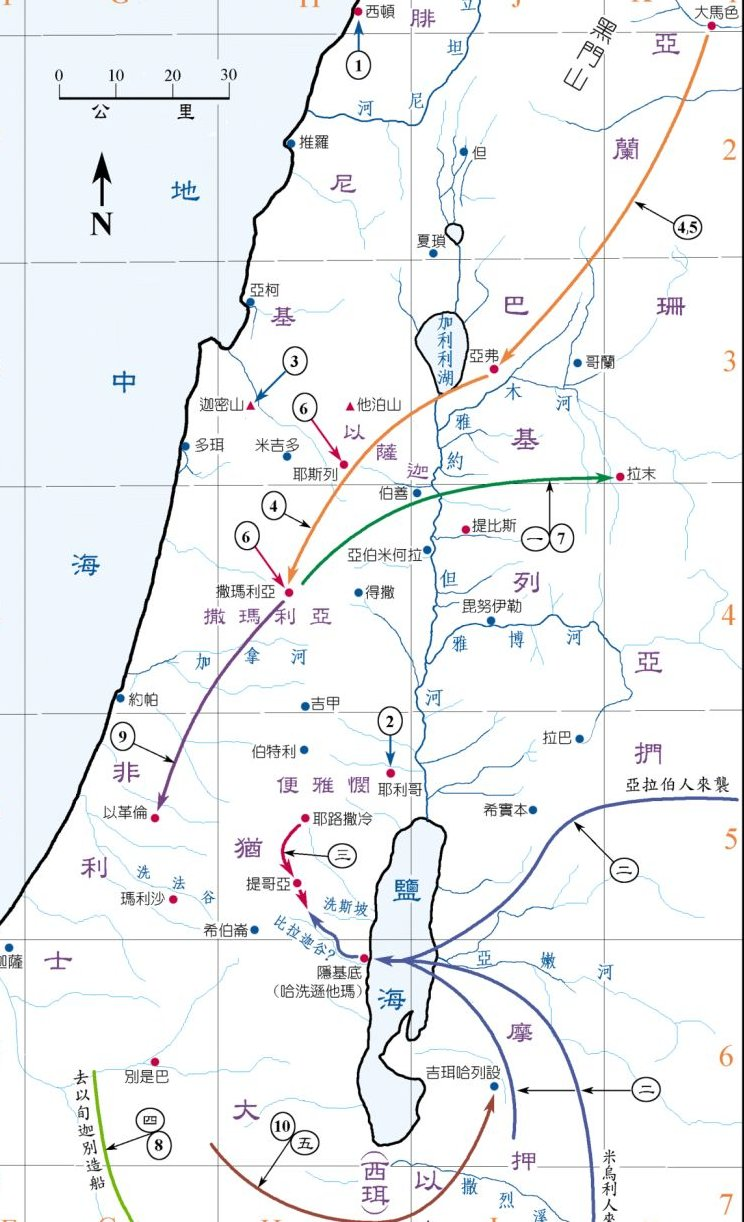
\includegraphics[width=3.8in]{BLiShiFigs/king/jilie}
\caption{亞比雅與耶羅波安爭戰}
\label{fig:sub1}
\end{figure}

\section{猶大王 - 約沙法 22:41-50 }
以色列王亞哈第四年，亞撒的兒子約沙法登基做了猶大王。 42 約沙法登基的時候年三十五歲，在耶路撒冷做王二十五年。他母親名叫阿蘇巴，乃示利希的女兒。 43 約沙法行他父親亞撒所行的道，不偏離左右，行耶和華眼中看為正的事。只是丘壇還沒有廢去，百姓仍在那裡獻祭燒香。 44 約沙法與以色列王和好。

45 約沙法其餘的事和他所顯出的勇力，並他怎樣爭戰，都寫在《猶大列王記》上。 46 約沙法將他父親亞撒在世所剩下的孌童都從國中除去了。 47 那時以東沒有王，有總督治理。 48 約沙法製造他施船隻，要往俄斐去，將金子運來。只是沒有去，因為船在以旬迦別破壞了。 49 亞哈的兒子亞哈謝對約沙法說：「容我的僕人和你的僕人坐船同去吧。」約沙法卻不肯。 50 約沙法與列祖同睡，葬在大衛城他列祖的墳地裡。他兒子約蘭接續他做王。
%\subsection{約沙法登基作王 22:41-42 }
%\subsection{約沙法作王做王与亚哈交好 22:43-50 }

\section{以色列王 - 亞哈謝 22:51-53 }
%\subsection{亞哈謝在撒玛利亚登基作以色列王 22:51 }
%\subsection{亞哈謝作以色列王行恶 22:52-52 } 
猶大王約沙法十七年，亞哈的兒子亞哈謝在撒馬利亞登基，做以色列王共二年。 52 他行耶和華眼中看為惡的事，效法他的父母，又行尼八的兒子耶羅波安使以色列人陷在罪裡的事。 53 他照他父親一切所行的，侍奉敬拜巴力，惹耶和華以色列神的怒氣。



  





